\documentclass{sig-alternate-05-2015}

% Fix to revert the changes IEEEtran makes to table caption styles
\usepackage{etoolbox}
\makeatletter
\patchcmd{\@makecaption}
  {\scshape}
  {}
  {}
  {}
\makeatother

%===========================================================================
\usepackage{listings}
\lstloadlanguages{C++}

% Settings for the lstlistings environment
\lstset{
language=C++,                       % choose the language of the code
basicstyle=\footnotesize\ttfamily,  % the size of the fonts that are used for the
                                    % code
numbers=none,                       % where to put the line-numbers
numberstyle=\tiny,                  % the size of the fonts that are used for the
                                    % line-numbers
stepnumber=1,                       % the step between two line-numbers. If it's
                                    % 1 each line will be numbered
numbersep=5pt,                      % how far the line-numbers are from the code
%backgroundcolor=\color{gray},      % choose the background color. You must add
                                    % \usepackage{color}
showspaces=false,                   % show spaces adding particular underscores
showstringspaces=false,             % underline spaces within strings
showtabs=false,                     % show tabs within strings adding particular
                                    % underscores
keywordstyle=\bfseries\color{blue},  % color of the keywords
commentstyle=\color{darkgreen},     % color of the comments
stringstyle=\color{darkred},        % color of strings
captionpos=b,                       % sets the caption-position to top
tabsize=2,                          % sets default tabsize to 2 spaces
frame=tb,                           % adds a frame around the code
breaklines=true,                    % sets automatic line breaking
breakatwhitespace=false,            % sets if automatic breaks should only happen
                                    % at whitespace
escapechar=\%,                      % toggles between regular LaTeX and listing
belowskip=0.3cm,                    % vspace after listing
morecomment=[s][\bfseries\color{blue}]{struct}{\ },
morecomment=[s][\bfseries\color{blue}]{class}{\ },
morecomment=[s][\bfseries\color{blue}]{public:}{\ },
morecomment=[s][\bfseries\color{blue}]{public}{\ },
morecomment=[s][\bfseries\color{blue}]{protected:}{\ },
morecomment=[s][\bfseries\color{blue}]{private:}{\ },
morecomment=[s][\bfseries\color{black}]{operator+}{\ },
xleftmargin=0.1cm,
%xrightmargin=0.1cm,
}

\usepackage{color}
\usepackage{comment}
\usepackage{graphicx}
\usepackage{subfig}
\usepackage{multirow}

\usepackage{rotating}
\usepackage{pdflscape}

\captionsetup[subfigure]{position=top}

%\usepackage[font=scriptsize,justification=justified,singlelinecheck=false]{caption}

\usepackage{array}

\makeatletter
\newcommand{\thickhline}{%
    \noalign {\ifnum 0=`}\fi \hrule height 1pt
    \futurelet \reserved@a \@xhline
}
\newcolumntype{"}{@{\hskip\tabcolsep\vrule width 1pt\hskip\tabcolsep}}
\makeatother

\usepackage{amsmath}
\usepackage{amsfonts}
\usepackage[hidelinks]{hyperref}
\usepackage{cite}

\usepackage{diagbox}

\usepackage{soul}% for hl
\usepackage{xcolor}% for background highlighting with \colorbox or \textcolor

\usepackage{fixme}
\fxusetheme{color}
\fxsetup{
    status=draft,
    author=,
    layout=inline, % also try footnote or pdfnote
    theme=color
}

\definecolor{fxnote}{rgb}{0.8000,0.0000,0.0000} % red
\colorlet{fxnotebg}{yellow}

\makeatletter
\renewcommand*\FXLayoutInline[3]{%
  \@fxdocolon {#3}{%
    \@fxuseface {inline}%
    \begingroup
      \sethlcolor{fx#1bg}%
      \color {fx#1}\ignorespaces \hl{#3\@fxcolon #2}%
    \endgroup%
  }%
}
\makeatother

\makeatletter
\renewcommand*\FXLayoutMargin[3]{%
  \marginpar[%
    \@fxdocolon {#3}{%
      \raggedleft%
      \@fxuseface {margin}%
      \begingroup
        \sethlcolor{fx#1bg}%
        \color {fx#1}\ignorespaces \hl{#3\@fxcolon #2}%
      \endgroup%
    }%
  ]{%
    \@fxdocolon {#3}{%
      \raggedright%
      \@fxuseface {margin}%
      \begingroup
        \sethlcolor{fx#1bg}%
        \color {fx#1}\ignorespaces \hl{#3\@fxcolon #2}%
      \endgroup%
    }%
  }%
}
\makeatother

%\newcommand{\fxnote}[1]{\fxnote{\colorbox{yellow}{\color{red}#1}}}
%\newcommand{\fxnotefootnote}[1]{\fxnote[footnote]{\colorbox{yellow}{\color{red}#1}}}

% Make fxnote footnotes have a background color and text color
\renewcommand\thefootnote{\colorbox{yellow}{\color{red}\arabic{footnote}}}

\pagenumbering{arabic}

%\linespread{2}

\usepackage{gitinfo2}
\usepackage{datetime}

%===========================================================================
\begin{document}
\title{Solving Large Quantities of Small Matrix Problems on Cache-Coherent SIMD Architectures}

%===========================================================================
% author names and affiliations
% use a multiple column layout for up to three different
% affiliations
\numberofauthors{1}
\author{
\alignauthor
Bryce Adelstein Lelbach, Hans Johansen, and Samuel Williams\\
\affaddr{Lawrence Berkeley National Laboratory, Computational Research Division}\\
\email{{\it \{balelbach, hjohansen, swwilliams\}@lbl.gov}}\\
{\small Revision \gitAbbrevHash \gitReferences, Built at \currenttime \vspace{1ex} on \today}
}
% \IEEEauthorblockN{Bryce Adelstein Lelbach, Hans Johansen, and Samuel Williams}
% \IEEEauthorblockA{Computational Research Division, Lawrence Berkeley National Laboratory, Berkeley, CA 94720\\ {\it \{balelbach, hjohansen, swwilliams\}@lbl.gov}}
%\and
%\IEEEauthorblockN{Homer Simpson}
%\IEEEauthorblockA{Twentieth Century Fox\\
%Springfield, USA\\
%Email: homer@thesimpsons.com}
% }

% conference papers do not typically use \thanks and this command
% is locked out in conference mode. If really needed, such as for
% the acknowledgment of grants, issue a \IEEEoverridecommandlockouts
% after \documentclass

% for over three affiliations, or if they all won't fit within the width
% of the page, use this alternative format:
% 
%\author{\IEEEauthorblockN{Michael Shell\IEEEauthorrefmark{1},
%Homer Simpson\IEEEauthorrefmark{2},
%James Kirk\IEEEauthorrefmark{3}, 
%Montgomery Scott\IEEEauthorrefmark{3} and
%Eldon Tyrell\IEEEauthorrefmark{4}}
%\IEEEauthorblockA{\IEEEauthorrefmark{1}School of Electrical and Computer Engineering\\
%Georgia Institute of Technology,
%Atlanta, Georgia 30332--0250\\ Email: see http://www.michaelshell.org/contact.html}
%\IEEEauthorblockA{\IEEEauthorrefmark{2}Twentieth Century Fox, Springfield, USA\\
%Email: homer@thesimpsons.com}
%\IEEEauthorblockA{\IEEEauthorrefmark{3}Starfleet Academy, San Francisco, California 96678-2391\\
%Telephone: (800) 555--1212, Fax: (888) 555--1212}
%\IEEEauthorblockA{\IEEEauthorrefmark{4}Tyrell Inc., 123 Replicant Street, Los Angeles, California 90210--4321}}




% use for special paper notices
%\IEEEspecialpapernotice{(Invited Paper)}




% make the title area
\maketitle

%===========================================================================

\begin{abstract}
A number of computational science algorithms lead to discretizations
  that require a large number of independent, small matrix solves.
Examples include small non-linear coupled chemistry and flow systems,
  one-dimensional sub-systems in climate and diffusion simulations, 
  alternating direction implicit pre-conditioners, and 
  semi-implicit time integrators, among others.
We present a performant approach for solving large quantities of 
  independent matrix problems on cache-coherent SIMD architectures.
Unlike many vectorized or ``batched'' approaches that rely on reusing
  the matrix factorization across multiple solves, our algorithm supports
  the case of sets of matrices that are different, due to
  spatial variation or non-linear solvers, for example.
We evaluate the performance of the approach with a benchmark 
  tridiagonal matrix solver that uses only OpenMP pragmas, tiling,
  and memory layouts to optimize memory bandwidth.
Performance is evaluated on Intel architectures with different cache,
  vectorization, and threading features (IVB, HSW, and KNL), 
  and compared to theoretical roofline models across parameter studies.
We conclude that the approach is effective at optimizing vectorization 
  and achieves $90\%$ of stream bandwidth on these architectures, 
  and improves on existing approaches (like LAPACK) for efficiently
  solving large numbers of small matrix problems.
\end{abstract}

% no keywords


% For peer review papers, you can put extra information on the cover
% page as needed:
% \ifCLASSOPTIONpeerreview
% \begin{center} \bfseries EDICS Category: 3-BBND \end{center}
% \fi
%
% For peerreview papers, this IEEEtran command inserts a page break and
% creates the second title. It will be ignored for other modes.
% \IEEEpeerreviewmaketitle

%===========================================================================
\section{Introduction}
\label{sec:introduction}

One important class of problems in computational science is the solving
  of smaller-dimensional matrix subproblems that are duplicated across
  many degrees of freedom in a larger two (or more) dimension computation.
Several examples of this include: 
\begin{itemize}
\item Pointwise chemistry systems in the context of a larger, 
  flow simulations. 
Examples include geochemistry~\cite{PFLOTRAN_2010}, 
  cloud microphysics~\cite{MG2_2015}, and combustion~\cite{PaznerEtAl_2016};
\item Solving one-dimensional systems that represent a numerically ``stiff''
  direction for a physical phenomenon.
Examples here include atmospheric radiation~\cite{RRTMG_2008}, groundwater
  penetration~\cite{CLM_PFLO_2016}, or models for 
  cloud convection~\cite{SAM_2005}; and
\item Implicit solvers that need to couple these kinds of subsystems, 
  such as line relaxation~\cite{TrottenbergEtAl_2000} and 
  semi-implicit time integrators~\cite{WellerEtAl_2013}.
\end{itemize}
In most cases, these matrices are relatively small 
  (ranging from \(O(10-100)\) chemistry components or ``levels'' 
  in a climate application), and may be sparse or dense, but must 
  be solved repeatedly, but with different entries each time, 
  to advance the overall simulation.
Thus, because these are often non-linear matrix systems with space- and 
  time-dependent entries, these applications may not use a 
  ``factor once, solve many times'' approach, which is often used 
  as a model matrix performance test.
This prevents amortizing setup and factorization costs across multiple
  right-hand side solves as in \lstinline{dptsv()}, \lstinline{dtsvb()},
  \lstinline{dgtsv()} and \lstinline{dgttrs()}~\cite{intel_mkl_manual}.
In that case, it is usually sub-optimal on SIMD many-core or SIMT GPGPU
  architectures to simply call an optimized linear algebra library, 
  such as Intel's Math Kernel Library (MKL)~\cite{mkl_website} or NVIDIA's
  CUDA Basic Linear Algebra Subroutines (cuBLAS)~\cite{cublas_website}; these
  may not achieve peak memory bandwidth and floating-point performance across 
  the range of small matrix size. 
In that sense, it can leads applications to create their own 
  custom implementations, which may not be optimal, and create a 
  (potentially unnecessary) maintenance burden for the applications 
  running across multiple many-core architectures as well. 
  
To this end, we have developed a model matrix kernel that mimics what
  is encountered in these kinds of large-scale simulations.
Key aspects of the code include:
\begin{itemize}
\item A three-dimensional application (that is, \((i,j,k)\) indices),
  where different matrix systems in the \emph{vertical} dimension \(k\) are
  generated at each \emph{horizontal} dimension \((i,j)\). 
\item Each matrix is tri-diagonal, and must be solved for all 
  \(nk \sim O(30-100)\) values in the \(k\) direction.
\item The matrix is derived from finite difference discretization for the
  1D diffusion equation, which allows it to be solved \emph{without pivoting}.
\end{itemize}
We note that pivoting and sparsity patterns are often application-specific;
  these requirements will be addressed in future work.

%===========================================================================
\section{Related Work}
\label{sec:related_work}

%{\color{red} TRIM AND MERGE UP \\
Approaches to solving large numbers of small matrices have been done
  in a variety of contexts.
Many implementations simply solve each matrix in parallel or for multiple
  right-hand sides, using platform-specific
  implementations of LAPACK, such as Intel's MKL or NVIDIA's cuBLAS implementations.
In many cases, there is a benefit from vectorization and thread parallelism, 
  but there may be overheads that reduce performance, such as data copies/
  temporary variables, 
  dynamic determination of optimal performance parameters, 
  and partially vectorized ``peel'' loops, for example.
Some specialized approaches include linear algebra-specific 
  compilers for small problem sizes and target architectures 
 ~\cite{Spampinato:2014, NelsonEtAl_2015}.
Other libraries like 
  \emph{Blaze}~\cite{BlazeSite}, 
  \emph{PLASMA}~\cite{PLASMASite},
  \emph{MAGMA}~\cite{Haidar:2015}, and 
  \emph{libxsmm}~\cite{libxsmm_website}
  are intended to support SIMD vectorization for standard vector sizes
  as well as batched computation for sparse and dense matrices.
Overall, there is a gap in approaches that have both effective vectorization,
  regardless of matrix size, with or without dense/sparse/pivoting 
  assumptions, amortizing factorization across multiple right-hand-sides, 
  and other assumptions.
%}
%===========================================================================
\section{Implementation}
\label{sec:implementation}

Suppose we have an \(nk \times nk\) tridiagonal matrix \(A\) and two \(nk\) element
  vectors \(u^{s}\) and \(u^{s+1}\).  We wish to solve \(Au^{s+1} = u^{s}\) for
  \(u^{s+1}\):

\[
\begin{bmatrix}
b_0 & c_0 &     &          & 0        \\
a_1 & b_1 & c_1 &          &          \\
    & a_2 & b_2 & ...      &          \\
    &     & ... & ...      & c_{nk-2} \\
0   &     &     & a_{nk-1} & b_{nk-1}
\end{bmatrix}
\begin{bmatrix}
u^{s+1}_0     \\
u^{s+1}_1     \\
...     \\
...     \\
u^{s+1}_{n-1}
\end{bmatrix}
=
\begin{bmatrix}
u^{s}_0     \\
u^{s}_1     \\
...     \\
...     \\
u^{s}_{n-1}
\end{bmatrix}
\]

Our matrix \(A\) is stored as a set of three vectors: an \(nk-1\) element
  sub-diagonal vector \(a\), an \(nk\) element diagonal vector \(b\) and an
  \(nk-1\) element super-diagonal vector \(c\).
In practical applications, a different matrix \(A\) exists for each \((i,j)\)
  location, because the diagonals may depend on the previous solution \(u^{s}\)
  (in a non-linear iteration loop, for example).

% Overview of SSTA solver.
We present the Simultaneous Streaming Thomas Algorithm (SSTA), a tridiagonal
  matrix solver based on the Thomas
  algorithm~\cite{ConteEtAlElementaryNumericalAnalysis,QuarteroniEtAl2007,TDMA}
  which was designed to solve large quantities of relatively small (\(O(30-100\))
  systems efficiently if they are \emph{diagonally-dominant}, which avoids
  the need for pivoting.
The SSTA solver computes the solution to multiple systems simultaneously, facilitating
  the use of vector instructions.
Additionally, SSTA iterates through memory in unit stride to enable software and 
  hardware prefetching facilities to easily track the data streams used in the solver.
We compare performance against STREAM Triad~\cite{stream} and a baseline solver
  derived from a production climate code which utilizes the Intel Math Kernel
  Library (MKL) and exposes task parallelism, but solves each matrix
  independently and does not utilize vector processing capabilities.

\subsection{The Thomas Algorithm}
\label{sec:implementation:thomas_algorithm}

With the assumption of a \emph{diagonally-dominant} tridiagonal matrix, 
  we can use a simplified
  form of Gaussian elimination that does not require pivoting, known as the
  Thomas algorithm or the tridiagonal matrix algorithm
  (TDMA)~\cite{ConteEtAlElementaryNumericalAnalysis,QuarteroniEtAl2007,TDMA}. 
This takes advantage of sparsity to be \(O(nk)\) in time, 
  and can be extended to banded matrices and LU factorizations.
It is also a significant improvement over dense Gaussian elimination,
  which is \(O(nk^3)\) in time. 
We use a formulation of the Thomas algorithm which does not require any storage
  for temporary values but overwrites the \(b\) vector and solves for \(u^{s+1}\)
  in-place, overwriting \(u^{s}\).

The Thomas algorithm consists of two passes.  First, a forward pass is
  performed to eliminate the \(a_i\) elements:
\begin{lstlisting}
for (auto k = 1; k < nk; ++k) {
  auto const m = a[k] / b[k - 1];
  b[k] -= m * c[k - 1];
  u[k] -= m * u[k - 1];
} 
\end{lstlisting}
Then, an abbreviated form of backwards substitution is performed to obtain the
  solution:
\begin{lstlisting}
u[nk - 1] = u[nk - 1] / b[nk - 1];

for (auto k = nk - 2 ; k >= 0; --k) {
  u[k] = (u[k] - c[k] * u[k + 1]) / b[k];
} 
\end{lstlisting}

The Thomas algorithm is a very low algorithmic intensity (AI)~\cite{roofline}
  algorithm.
During the course of our work, we developed a theoretical peak performance
  model for the Thomas algorithm.
First, we count the number of FLOPs performed.
We will consider multiplications, additions and division operations as FLOPs.

Each iteration of the forward elimination loop contains 1 division, 2
  multiplications and 2 subtractions.
This gives us a total of either \(3(nk-1)\) FLOPs on fused-multiply-add (FMA)
  architectures~\cite{intel_fma_website} or 
  \(5(nk-1)\) FLOPs on non-FMA architectures.
Next, the pre-substitution operation (the assignment to \lstinline{u[nk - 1]}
  in the above snipper) performs a single division.
Finally, the backwards substitution loop, performs 1 multiplication, 1
  subtraction and 1 division, adding either \(2(nk-1)\) FLOPs (FMA architectures)
  or \(3(nk-1\) FLOPs (non-FMA architectures).
In total, this gives us either \(5nk-4\) FLOPs (FMA) or \(8nk-7\) FLOPs
  (non-FMA) for the entire Thomas algorithm.

Our data movement model for the Thomas algorithm assumes that we will achieve
  optimal performance when data is cached between the forward elimination and
  back substitution loop.
That is, we assume that accesses to \(a\), \(b\), \(c\) and \(u\) will
  \emph{not} go to main memory in the back substitution loop because the arrays
  still remain in cache from the forward elimination loop accesses.

The Thomas algorithm accesses four arrays, reading from all of them (\(a\),
  \(b\), \(c\) and \(u\)) and writing to two of them (\(b\), \(u\)).
\(b\) and \(u\) have extent \(nk\), so we write \(2nk\) elements.
\(a\) and \(c\) have extent \(nk-1\), so we read \(2(nk-1)+2(nk)\) elements.
In total, \(6nk-2\) elements are moved.
Assuming double precision, \(48nk-16\) bytes are moved from main memory
  during execution of the Thomas algorithm.

We verified our analytic model by measuring hardware performance counters which
  track memory traffic with the Intel VTune Amplifier
  profiler~\cite{intel_vtune_amplifier}.
We found that memory bandwidth measured via hardware counters generally agreed
  with effective bandwidth computed using our analytic model.

This gives us a FLOPs/byte ratio of \((5nk-4)/(48nk-16)\) (FMA) or
  \((8nk-7)/(48nk-16)\) (non-FMA).
The lower bound for the Thomas algorithm's arithmetic intensity is \(1/32\)
  FLOPs/byte when \(nk=1\). 
The upper bound is \(5/48\) FLOPS/byte (FMA) or \(1/6\) FLOPs/byte (non-FMA) as
  \(nk\) approaches infinity.
Based on this analytic analysis, we can conclude that the Thomas algorithm is
  \emph{memory-bandwidth bound}.

\subsection{Batching and Vectorization}
\label{sec:implementation:batching_and_parallelism}

\begin{figure*}[!bt]
  \centering
  \caption{
    \textbf{Independent Solve Strategy:} A vertical column of \(nk\) elements is
      extracted from a \(ni \times nj \times nk\) 3D Cartesian grid and used as
      the right-hand side in a tridiagonal linear system.
    The system for each column is solved independently from other columns.
    This approach exposes task parallelism, but vectorization is not possible
      in the vertical dimension \(k\) due to its small extent and loop-carried
      dependencies present in Thomas algorithm.
  }
  \label{fig:implementation:independent_solve_strategy}
  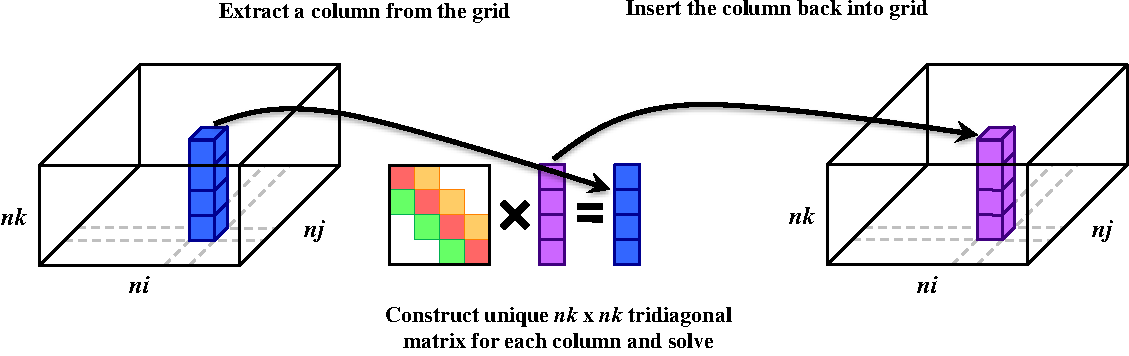
\includegraphics[width=0.95\textwidth]{figures/independent_solve.pdf}
\end{figure*}

\begin{figure*}[!bt]
  \centering
  \caption{
    \textbf{Simultaneous Solve Strategy:} A tile of vertical columns, each 
      containing \(nk\) elements, is extracted from a \(ni \times nj \times nk\)
      3D Cartesian grid and used as the right-hand side in a tridiagonal linear
      system.
    All the columns in the tile are solved simultaneously.
    This approach exposes task parallelism, exhibits good data locality and
      enables vectorization in one of the horizontal dimensions (\(i\)).
  }
  \label{fig:implementation:simultaneous_solve_strategy}
  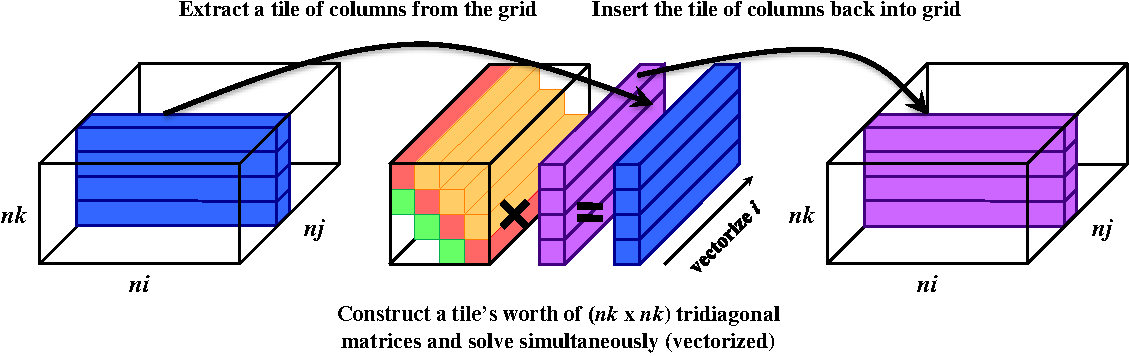
\includegraphics[width=0.95\textwidth]{figures/simultaneous_solve.pdf}
\end{figure*}

In the applications described in \S\ref{sec:introduction} we need to apply the
  Thomas algorithm to each vertical column in a \(ni \times nj \times nk\)
  Cartesian grid, where \(i\) and \(j\) are horizontal dimensions and \(k\) is
  the vertical index.
These computations are known as the \emph{vertical solves}.
Since each vertical solve is independent of the others, this is an
  embarrassingly parallel problem.
The matrix coefficients for each column depend on the problem state, so a
  unique matrix for each column needs to be constructed before each solve.
There are two different approaches to computing these batch solves.

The most straightforward approach is \emph{solve} each column
  \emph{independently} (the \emph{independent solve strategy}; Figure
  \ref{fig:implementation:independent_solve_strategy}).
An \(nk \times nk\) tridiagonal matrix is constructed for each column, and then
  the Thomas algorithm is used to solve the system formed by the matrix and the
  vertical column.
Because the vertical solves are independent, they can be executed concurrently
  via task-level parallelism.
Vectorization of the \(nk\) loop is not possible as each iteration of the loops
  in the Thomas algorithm is dependent on the previous iteration (e.g.
  loop-carried dependency)~\cite{povitsky}.
Although the LAPACK interface contains no routine for Thomas algorithm,
  \lstinline{dgtsv()} and \lstinline{dgttrs()} (which solve tridiagonal and
  banded systems, respectively) use this approach.

The other approach is to \emph{simultaneously solve} multiple columns (the
  \emph{simultaneous solve strategy}; Figure
  \ref{fig:implementation:simultaneous_solve_strategy}).
A block \(nk \times nk\) tridiagonal matrix is constructed for the whole grid;
  each block contained within the matrix is an \(ni \times nj\) horizontal plane
  (e.g. the block matrix is a 4D space).
To perform the vertical solves, we view the entire 3D Cartesian grid as an
  \(nk\) block vector of \(ni \times nj\) planes and apply it to the block
  matrix.
Each step of the algorithm is applied across an entire plane.
For example, the forward sweep becomes:
\begin{lstlisting}
for (auto k = 1; k < nk; ++k)
for (auto j = 0; j < nj; ++j)
for (auto i = 0; i < ni; ++i) {
  auto const m = a[i][j][k]
               / b[i][j][k - 1];
  b[i][j][k] -= m * c[i][j][k - 1];
  u[i][j][k] -= m * u[i][j][k - 1];
} 
\end{lstlisting}
This approach facilities both task-level parallelism and vectorization.
The grid and block matrix can be tiled into smaller subgrids, and the Thomas
  algorithm can be applied to each subgrid independently.
Each step of the Thomas algorithm can be vectorized across the \(ni \times nj\)
  horizontal plane that it is operating on: e.g. the \(i\) or \(j\) loops in the
  above snippet can be vectorized.
For the SSTA solver, the horizontal dimension \(i\) is always the unit stride
  dimension, and the direction in which we vectorize.

%\fxnote{TODO: Explain that the independent solve approach is what LAPACK does,
%and that's why it is insufficient for this type of problem. Also, explain that
%LAPACK has no routine for Thomas-style tridiagonal solves - dgtsv is
%generalized, does actual Gaussian eliminiation and may do pivoting. Also
%mention somewhere that MKL does not parallelize dgtsv.}

%{\color{red} CUT REDUNDANT WITH INTRO \\
The vector parallelism exposed by the simultaneous approach offers a major
  benefit over the independent approach, since it is not possible to vectorize
  most of the kernels in the independent approach due to data dependencies
  between iterations of the Thomas algorithm.
Even if it was possible to vectorize in the vertical \(nk\) dimension, it would
  still be undesirable to do so.
The extent of the vertical dimension tends to be very small in the applications
  we are concerned with \(O(30-100)\).
Vectorizing in the horizontal dimensions allows us to control locality and loop
  trip counts via tiling.
%}

\subsection{Data Layout}
\label{sec:implementation:data_layout}

The data layout of the Cartesian grid has a huge impact on the performance
  potential of the vertical solves.
Throughout the course of our research, our understanding of the impact of
  different data layouts has evolved substantially.
We have investigated three different schemes:
\begin{table}[h]
\centering
% NOTE: kji AKA column-major, Fortran, left
% NOTE: ijk AKA row-major, C++, right
%\caption{\textbf{Data Layouts for the 3D Cartesian Grid:} The following three
%data layouts were investigated in the course of this research. The \(kji\)-layout
%is optimal for the independent solve strategy. The \(ijk\)-layout is effective
%for the simultaneous solve strategy, but the \(ikj\)-layout provides better
%data locality (\S\ref{lab:tiling}) and out performs the \(ijk\)-layout on
%Knight's Landing (Figure \ref{})}
\caption{\textbf{Data Layouts for the 3D Cartesian Grid}}
\begin{tabular}[t]{|c|c|c|c|} \hline
\textbf{Name}         & \textbf{\(i\)-stride} & \textbf{\(j\)-stride} & \textbf{\(k\)-stride}   \\\cline{2-3}
                      & \multicolumn{2}{c|}{\textbf{(Horizontal)}}                 & \textbf{(Vertical)} \\ \hline
\(ijk\), Column-Major & \(1\)             & \(ni\)            & \(ni * nj\)         \\ \hline
\(kji\), Row-Major    & \(nj * nk\)       & \(nk\)            & \(1\)               \\ \hline
\(ikj\)               & \(1\)             & \(ni * nz\)       & \(ni\)              \\ \hline
\end{tabular}
\label{tab:implementation:data_layout:layouts}
\end{table}

The production code that our MKL baseline solver is derived from uses the
  \(ijk\)-layout.
The vertical columns that we need to pass in to MKL as the solution vector
  (\(u\)) are non-contiguous, as the vertical dimension \(k\) is the dimension
  with greatest stride.
Currently, the production codebase allocates a temporary gather buffer, copies
  data from the grid into the buffer, calls the LAPACK solver, and then copies
  the result from the buffer back to the grid.

%{\color{red} CUT-MERGE LEARNINGS IN NEXT \S~\ref{sec:tiling} \\
We have found the \(kji\)-layout to be optimal for our MKL baseline solver.
With the \(kji\)-layout, we have contiguous vertical columns which can be
  passed to MKL without temporary allocations or unnecessary copies.
We observed a noticeable performance increase from this change with very
  little source code impact, although we have not studied the impact of this
  layout change on horizontal solver components.

%Eventually, we determined that LAPACK would not be sufficient for the vertical
%solves and that we could achieve substantially higher bandwidths by developing
%the solver described in this paper, we revisited the data layout question. As
%we would not be able to vectorize the Thomas algorithm in the vertical
%dimension due to the the loop-carried dependencies present in the algorithm, we
%decided to switch back to an \(ijk\) layout, where one horizontal dimension (\(i\))
%is the unit stride dimension and the vertical dimension (\(k\)) has the greatest
%stride.

Our SSTA solver uses either the \(ijk\)- or \(ikj\)-layout.
The SSTA algorithm vectorizes in one of the horizontal directions (as described
  in \S\ref{sec:implementation:batching_and_parallelism}), so it is desirable to
  use layouts where the horizontal dimension that we are vectorizing (\(i\)) is
  the unit stride dimension, avoiding strided vector loads.
The \(ikj\) layout arose as an optimization to combat data locality and prefetching
  issues which hindered performance on the Intel Xeon Phi Knight's Landing
  architecture, and is described in greater detail in the following section.
%}

\subsection{Tiling}
\label{sec:implementation:tiling}

\begin{figure}[!bt]
  \centering
  \caption{
    \textbf{Tile-\(j\) Scheme with the \(ijk\)-Layout:} 
    Unit stride in \(i\) then \(j\) directions, creating a tile from an 
    \(ni \times mj \times nk \) plane, where \(1 \le  mj \le nj \).
    Note that memory is not contiguous in the \(k\) direction; 
    colors indicate strides of $O(ni \times nj)$.
    \fxnote{Bryce: review?}
  }
  \label{fig:implementation:tiling:ijk_layout_tile_j}
  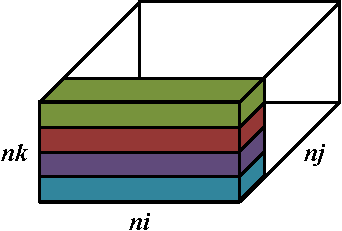
\includegraphics[width=0.70\columnwidth]{figures/ijk_layout_tile_j_scheme.pdf}
  \vspace{-.5cm}
\end{figure}

\begin{figure}[!bt]
  \centering
  \caption{
    \textbf{Tile-\(ij\) Scheme with the \(ijk\)-Layout:} 
    Unit stride in \(i\) then \(j\) directions, creating a tile from an 
    \(mi \times mj \times nk \) block, 
    where \(1 \le  mi \le ni \) and \(1 \le  mj \le nj \).
    Note that memory is not contiguous in \(k\) here as well.
    \fxnote{Bryce: review?}
  }
  \label{fig:implementation:tiling:ijk_layout_tile_ij}
  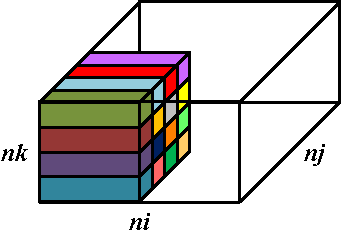
\includegraphics[width=0.70\columnwidth]{figures/ijk_layout_tile_ij_scheme.pdf}
  \vspace{-.5cm}
\end{figure}

\begin{figure}[!bt]
  \centering
  \caption{
    \textbf{Tile-\(j\) Scheme with the \(ikj\)-Layout:}
    Unit stride in \(i\) then \(k\) directions, creating a tile from an 
    \(ni \times mj \times nk \) block, where \(1 \le  mj \le nj \).
    Note that memory is contiguous in the tile.
    \fxnote{Bryce: review?}
  }
  \label{fig:implementation:tiling:ikj_layout_tile_j}
  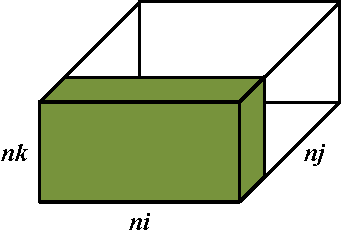
\includegraphics[width=0.70\columnwidth]{figures/ikj_layout_tile_j_scheme.pdf}
  \vspace{-.5cm}
\end{figure}

\begin{figure}[!bt]
  \centering
  \caption{
    \textbf{Tile-\(ij\) Scheme with the \(ikj\)-Layout:}
    Unit stride in \(i\) then \(k\) directions, creating a tile from an 
    \(mi \times mj \times nk \) block, where \(1 \le  mi \le ni \)
    and \(1 \le  mj \le nj \).
    Note that memory is contiguous in planes, but strided by $O(ni \times nk)$.
    \fxnote{Bryce: review?}
  }
  \label{fig:implementation:tiling:ikj_layout_tile_ij}
  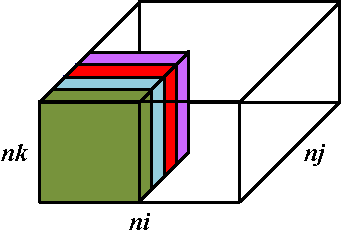
\includegraphics[width=0.70\columnwidth]{figures/ikj_layout_tile_ij_scheme.pdf}
  \vspace{-.5cm}
\end{figure}

To ensure good CPU cache utilization, it is often necessary to break a larger
  grid into smaller \textbf{tiles} which better amortize nested loop overheads, expose
  greater data locality and keep data resident in a particular level of the
  cache hierarchy~\cite{blocked_algorithms}.
This technique is also known as \textbf{cache blocking}.
Additionally, partitioning a grid with dimensions known at application
  initialization into fixed size tiles can provide some of the performance
  benefits of compile-time-fixed dimensions (e.g. compiler optimizations) with
  the flexibility of a dynamically sized problem~\cite{kokkos}.
Tiling also provides a useful abstraction for task parallelization, as
  each tile can be computed independent of other tiles and has no overlapping
  data accesses.
Tiling is particularly important for memory-bandwidth bound computations like
  tridiagonal matrix solves.

The production code which our MKL baseline solver is derived from is not task
  parallelized or explicitly tiled.
Since each column is solved independently, there is little opportunity to improve
  locality and reuse via tiling.
Conceptually, since each column is solved independently in the production code,
  it is \emph{effectively} tiled, albeit with a very small tile size (a single
  column, e.g. \(O(nk) \sim O(30-100)\)).
Our MKL baseline solver is tiled solely to facilitate task parallelization.

On the other hand tiling is very fundamental to our SSTA solver.
Our analytical performance model (\S\ref{sec:implementation:thomas_algorithm})
  is based on caching assumptions which we rely on tiling to enforce.
In particular, we assume that all four arrays (\(a\), \(b\), \(c\) and \(u\))
  to remain in the cache hierarchy in between the forward elimination and the
  back substitution loops.
On x86-64 SIMD architectures, we typically aim to fit within the L2 cache.
If any of these four arrays need to be reloaded from main memory in between the
  forward elimination and back substitution loops, the amount of main memory data
  movement is significantly increased and the algorithmic intensity of the
  algorithm decreases dramatically.
While our untiled SSTA results outperform the MKL baseline results (Figure
  \ref{fig:results:efficiency}), they were well below the manufacturer-specified
  bandwidth and STREAM~\cite{stream} Triad effective bandwidth.

Because it is necessary for all four arrays to remain in the cache hierarchy, 
  it is important to note the distinction between \textbf{per-array tile size}
  (e.g. the tile size for one of the four arrays) and the
  \textbf{total tile size} (e.g. the sum of the per-array tile sizes).
The total tile size is the amount of data we need to remain in cache in between
  the forward elimination and back substitution loops.

\fxnote{Use total tile size/per-array tile size from this point forward}

Due to the loop-carried dependencies in the Thomas algorithm and the small
  extent of \(nk\), we could not tile the vertical dimension. So, we explored two
  tiling schemes which partition the horizontal space.

%{\color{red} CUT MOST OF DISCUSSION, JUST STATE OPTIONS \\
The \textbf{tile-\(ij\)} scheme partitions both the \(i\) and \(j\) dimensions,
  yielding tiles with arbitrary horizontal shape. 
The \textbf{tile-\(j\)} scheme partitions only the \(j\) dimension, producing
  tiles of containing some of number of complete \(i\) (unit-stride) lines.
There is a trade-off between these two schemes, with the tile-\(ij\) scheme
  offering greater flexibility in tile size and the tile-\(j\) scheme offering
  greater contiguity. 

For example, suppose we partition an \(ijk\)-layout grid into four tiles with
  both the tile-\(ij\) scheme (producing \(ni/2 \times ni/2 \times nk\) tiles)
  and the tile-\(i\) scheme (producing \(ni \times ni/4 \times nk\) tiles).
Both tiles have the same size, \(nk \times ni^2/4\) elements.
However, the tile-\(j\) scheme has much greater data contiguity.
For the tile-\(ij\) scheme, tiles contain are \(nk \times ni/2\) contiguous
  \(i\)-lines, each containing \(ni/2\) elements.
For the tile-\(j\) scheme, tiles contain are \(nk\) contiguous \(ij\)-planes,
  each containing \(ni^2/4\) elements.

While the tile-\(j\) scheme offers greater contiguity than the
  tile-\(ij\) in this example, the tile-\(j\) tiles are not a single contiguous
  memory region.
The only way to obtain completely contiguous tiles in the \(ijk\)-layout would
  be to tile the dimension with the greatest stride (\(k\)), which is not possible
  because we cannot partition the vertical dimension.

This limitation led us to the \(ikj\)-layout for the SSTA solver.
In this layout, the direction of vectorization (\(i\)) is still the unit stride
  dimension, avoiding strided loads and assisting hardware prefetching.
Additionally, the tile-\(j\) tiles are completely contiguous regions of memory,
  decreasing translation-lookaside buffer pressure, increasing locality for
  caching and further assisting hardware prefetching.

Consider switching to the \(ikj\)-layout in the prior example.
The tile-\(ij\) tiles would contain \(ni/2\) contiguous \(ik\)-planes, each
  containing \(nk \times ni/2\) elements.
The tile-\(j\) tiles would be one contiguous region containing
  \(nk \times ni^2/4\) elements.

%We have observed that the greater contiguity of the tile-\(j\) approach leads
%  to fewer strided memory accesses, improved hardware prefetching and fewer
%  translation lookaside buffer (TLB) entries needed per tile (discussed in
%  \S\ref{results} and shown in Figure \ref{ref:results:tile_size_knl} and
%  \ref{ref:results:efficiency}).

The only notable downside to the tile-\(j\) scheme is the loss of
  flexibility in tile sizes.
The smallest tile size for the tile-\(j\) scheme is a \(ni \times 1 \times nk\)
  tile (an \(i\)-line of columns), while the smallest tile size for the
  tile-\(ij\) scheme is a \(1 \times 1 \times z\) tile (a single column).
We have not found this restriction to be overly problematic.
If the extent of \(i\) was large enough that the sum of the minimum tile sizes of
  the arrays \(a\), \(b\), \(c\) and \(u\) was greater than the capacity of the
  cache that we wished to reside within, we could likely switch to the tile-\(ij\)
  scheme without experiencing performance degradation due to decreased locality.

The SSTA solver supports both the \(ijk\)- and \(ikj\)-layout.
The tile-\(j\) scheme is used with both layouts.

%===========================================================================
\section{Experimental Setup}
\label{sec:experimental_setup:}
We developed the Tridiagonal Solve Benchmarks (TSB) suite during the course of
  the research described in this paper~\cite{tsb_git}.
The TSB suite is freely available on Github under the Boost Software License,
  version 1.0.
Revision \fxnote{WHATEVER} contains the source code used for the experiments in
  this paper.
The benchmark suite has three major components: a multi-dimensional array
  abstraction, generic solver components and a test harness.

\subsection{Test Problem}
\label{sec:experimental_setup:test_problem}

%{\color{red} REPLACE WITH EXACT MATRIX / STENCIL \\
The benchmarks in TSB are based on solving, in each vertical column,
  a matrix derived from a simple finite difference stencil 
  for an ``implicit Euler'' time step of the diffusion equation,
  with a $u=0$ boundary condition.
For a dimensionless diffusion coefficient \(D > 0\), this
  produces a \emph{diagonally-dominant} tridiagonal matrix:
\begin{align*}
A = 
\begin{bmatrix}
1 + 3D & -D &     &          & 0        \\
-D & 1 + 2D & -D &          &          \\
    & ...& ...    & ...     &              \\
    &         & -D & 1 + 2D     & -D \\
0   &     &     & -D & 1 + 3D
\end{bmatrix}  
\end{align*}
An identical form of the problem is initialized in every vertical column of the
  3D grid, but the matrices are initialized every time.
%}

%{\color{red} THIS SHOULD BE MOVED UP INTO TILING /INTRO SECTION \\
%Square and cubic problems tend to have limited flexibility in how they can be
%decomposed into equally-sized chunks of work, which can be problematic for a
%benchmark where we wish to explore different degrees of parallelism and
%different tile sizes. Because the horizontal (ij) shape of the 3D grid in TSB
%has little significance, we decided to prefer a long rectangular grid, with
%fixed and small i and k extents and a long, variable j extent.

%It should be noted that the horizontal shape of the grid is not entirely
%arbitrary for NAMEFORALGO. In the tile-j scheme that we use, the extent of i controls the
%lower bound on the tile size and completely controls the loop trip count for
%the inner-most unit-stride loop. We cannot use the vertical extent as a
%tile-size control because the number of vertical levels is largely determined
%by the physics of the production code.
%}

%\subsection{Constant Parameters}
%\label{sec:experimental_setup:constant_parameters}
%
%%{\color{red} CONVERT TO SMALL TABLE IN APPENDIX \\
%We held most of the parameters of the test problem constant when producing the
%results presented in this paper. A summary of the constant parameters and the
%rationale behind their value follows.
%
%\begin{itemize}
%\item Double precision data types were used for all results. 
%\item The vertical extent nk and the horizontal extent ni were both set to 32
%elements. We wanted to pick a power of 2 for the dimension that we would be
%holding constant, so that we could ensure we would observe cache aliasing
%conflicts when we picked a power of 2 for nj. For nk, we believe 32 elements is
%a reasonable lower bound for the number of vertical levels that would be used
%in our production climate code. The production codebase currently uses boxes
%with horizontal extents which are somewhat greater than 32 (\(O(64-256)\)).
%However, since $ni$ dictates the minimum tile size in our tile-j scheme, we
%wanted to pick a smaller quantity to ensure that we were able to full explore
%the space of possible tile sizes. 
%\item The horizontal extent $nj$ was set to \(2^14*3^2=147456\). Our target Ivy
%Bridge platform (see Table \ref{tab:test_platforms}) has 12 processing units
%per socket, so it was necessary to ensure that nj was divisible by 3 so that we
%would have an even, static division of work among processing units after
%tiling. With ni and nk set as 32, this gives a \textbf{problem size} of ~4.429
%GB (e.g. the sum of the size of the four arrays a, b, c and u). Recall that we
%allocate nixnjxnk instead of nixnjx(nk-1) elements for the diagonal a and c to
%simplify our cache aliasing conflict mitigation approach. So, the
%\textbf{storage size} size is actually 4.5 GB (not including padding elements
%for cache aliasing conflict mitigation).
%\item The number of time steps (ns) was set to 4 per processing unit. For
%example, running on 1 processing unit on our Knight's Landing platform, the
%number of time steps would be set to 4. Running on all 64 processing units, the
%number of time steps would be set to 256. This was done to ensure that runs
%using different numbers of processing units would execute in roughly the same
%amount of time without varying the problem size (e.g. fixed \textbf{problem
%size} but varying \textbf{total work}).
%\item The diffusion coefficient (D) in the test problem was set to 0.1 and the
%frequency of the sine wave (N) in the initial conditions was set to 1. The
%timestep size was set to 1e-7.
%\item ArrayBaseAlign was set to 1MB. On our Ivy Bridge and Haswell platforms,
%ArrayAlignStep was computed as 9216 bytes and PlanePadding was computed as 1152
%bytes. On our Knight's Landing platform, ArrayAlignStep was computed as 17408
%bytes and PlanePadding was computed as 2176 bytes. The plane padding storage
%overhead (\(nz*PlanePadding\)) on Ivy Bridge/Haswell was 36KB. On Knight's
%Landing it was 68KB.
%\end{itemize}
%%}
%
%The independent variables in our experiments were tile size (controlled by tile
%width), number of processing units (discussed below in Section \ref{}) and
%solver variant. The next section discusses the different solver strategies
%available in TSB, a subset of which were used in the experiments described in
%this paper.
%
%%{\color{red} CONVERT TO TABLE IN APPENDIX \\
%\subsection{TSB Variants}
%\label{sec:experimental_setup:tsb_variants}
%
%\begin{table*}%[t]
%\centering
%\caption{\textbf{Characterstics of the Tridiagonal Solve Benchmarks (TSB):}}
%%* for simultanous refers to the "merged" approach which can't be parallelized right now because
%\begin{tabular}{|c|c|c|c|} \hline
%\textbf{Characterstic}       & \textbf{Options}                                     \\ \hline
%Matrix Solver Family         & LAPACK, SSTA                                         \\ \hline
%Batching Strategy            & Independent (LAPACK), Simultaneous (SSTA, LAPACK*)   \\ \hline
%Floating Point Precision     & Single, Double (LAPACK, SSTA)                        \\ \hline 
%Layout                       & kji (LAPACK), ijk (SSTA, LAPACK), ikj (SSTA)         \\ \hline
%Tiling Scheme                & Tile J (SSTA, LAPACK), Tile IJ (SSTA*, LAPACK*)      \\ \hline
%Grid Type                    & Full, Rolling (SSTA, LAPACK)                         \\ \hline
%Parallel Programming Model   & OpenMP (SSTA, LAPACK), HPX (SSTA*)                   \\ \hline
%Thomas Algorithm Formulation & Repeated Divide, Cached Divide (SSTA)                \\ \hline
%Division Mechanism           & C++ Operator (SSTA, LAPACK), RCPPS w/ NR (SSTA)      \\ \hline
%\end{tabular}
%\label{tab:tsb_variant_characterstics}
%\end{table*}
%
%The TSB suite contains variants of two different families of tridiagonal matrix
%solvers: LAPACK-based variants which solve each vertical column independently, and
%NAMFORALGO variants. The distinguishing characteristics of the variants are
%listed in Table \ref{tab:tsb_variant_characterstics}. Each specific variant is
%instantiated by combining different generic building blocks within the TSB
%codebase; code which is shared by different variants is not duplicated.
%
%The list of possible variant instantiations is long and combinatoric in nature;
%we omit it for brevity, as the description of distinguishing characteristic is
%sufficiently descriptive.
%%}

\subsection{Hardware Platforms}
\label{sec:experimental_setup:hardware_platforms}

%{\color{red} MOVE TO APPENDIX/README \\
%\begin{table*}[t]
%\centering
%\caption{\textbf{Test Platforms:}}
%\begin{tabular}{|c|c|c|c|} \hline
%\textbf{System Name}     & \textbf{Edison}          & \textbf{Cori}            & \textbf{Carl}             \\ \hline
%Model                    & Intel Xeon E5-2695 v2    & Intel Xeon E5-2698 v3    & Intel Xeon Phi 7210       \\ \hline
%Microarchitecture        & Ivy Bridge               & Haswell                  & Knight's Landing          \\ \hline
%Vector Instruction Set   & AVX                      & AVX2                     & AVX512                    \\ \hline
%CPU Clock Frequency      & 2.4 GHz (3.2 GHz Turbo)  & 2.3 GHz (3.6 GHz Turbo)  & 1.3 GHz (1.5 GHz Turbo)   \\ \hline
%Processing Units (Cores) & 12                       & 16                       & 64                        \\ \hline
%Hardware Threading       & 2-way                    & 2-way                    & 4-way                     \\ \hline
%L1D Cache                & 32KB 8-way               & 32KB 8-way               & 32KB 8-way                \\
%                         & (local to each PU)     & (local to each PU)     & (local to each PU)      \\ \hline
%L2 Cache                 & 256KB 8-way              & 256KB 8-way              & 1024KB 16-way; 512KB/PU \\
%                         & (local to each PU)     & (local to each PU)     & (shared by 2 PUs)       \\ \hline
%L3 Cache                 & \fxnote{hwloc}           & \fxnote{hwloc}           & \fxnote{hwloc}            \\ \hline
%TLB                      & \fxnote{TODO}            & \fxnote{TODO}            & \fxnote{TODO}             \\ \hline
%DDR4 SDRAM               & \fxnote{TODO}            & \fxnote{TODO}            & \fxnote{TODO}             \\ \hline
%\end{tabular}
%\label{tab:test_platforms}
%\end{table*}

The TSB suite currently targets x86-64 microarchitectures with SIMD vector units
  running POSIX-compliant operating systems.
The results presented in this paper were collected from both Intel Xeon and
  Xeon Phi systems.

Our two Intel Xeon platforms, Edison~\cite{edison_configuration} and Cori Phase
  1~\cite{cori_phase_1_configuration}, are homogeneous Cray supercomputers,
  consisting of traditional dual-socket x86-64 processors.
Edison features Intel Xeon E5-2695 v2 Ivy Bridge (IVB)~\cite{intel_ark_xeon_e5_2695_v2}
  processors, and Cori Phase 1 has Intel Xeon E5-2698
  v3 Haswell (HSW)~\cite{intel_ark_xeon_e5_2698_v3} processors.
The Haswell microarchitecture offers a number of important improvements over
  Ivy Bridge relevant to the solver described in this paper, such as AVX2
  fused-multiply-add instructions, increased DDR4 memory bandwidth, increased
  cache bandwidth and other cache performance improvements~\cite{intel_opt_manual}.
However, in general, the two Xeon platforms have a very similar performance
  profile for our application.

Our Xeon Phi testbed, an Intel Xeon Phi 7210 Knight's Landing (KNL)~\cite{intel_ark_xeon_phi_7210}
  is notably different from the two Xeon systems.
It is a many-core design with a 2D mesh of \emph{light} cores optimized
  for throughput and explicit parallelism at the expense of increased latency
  and reduced complexity in other areas (branch prediction, out-of-order
  execution facilities, pipeline depth, etc).
The KNL microarchitecture has a number of novel features including on-package
  high-bandwidth MCDRAM (which can be used as programmable memory or a
  direct-mapped last-level cache), 4 hyper-threads per core and dual 512-bit
  AVX512 vector units.~\cite{roofline_knl,sodani_slides}

Knight's Landing processors can be configured for different Non-Uniform Memory
  Access (NUMA) topologies.
Additionally, the MCDRAM can be configured as programmable memory, a direct-mapped
  last-level cache or a combination of the two~\cite{sodani_slides}.
We used a \lstinline{quadcache} configuration, where all processing units are
  in a single NUMA domain and all 16GB of MCDRAM are used as a
  cache~\cite{roofline_knl}.

\subsection{Toolchain}
\label{sec:experimental_setup:toolchain}

TSB is written in ISO C++14 and has no external software dependencies.
The code contains no vector intrinsics or vector assembly.
We rely entirely on the compiler vectorization engine for performant vector code
  generation, utilizing compiler hints (via builtin functions and
  \lstinline{#pragma} directives) to guide vectorization indicate alignment, loop
  trip count and aliasing assumptions.
Avoiding vector intrinsics and hand-written assembly makes TSB performance
  portable between different x86-64 vector instruction sets (SSE, AVX, AVX2,
  AVX512) and simplifies porting to other architectures (such as SIMT GPUs).
We have also found it leads to better code generation by giving the compiler
  the freedom to select the correct instructions and perform optimizations which
  we have found to be inhibited by explicit vector intrinsics, such as
  post-vectorization loop unrolling.
Task parallelization is implemented using OpenMP
  \lstinline{#pragma}s~\cite{openmp}.
Since the problem is embarrassingly parallel in the horizontal dimensions, it
  is easy to statically load balance (dimension extents and tile sizes
  permitting).
The \emph{hwloc} affinity and topology framework~\cite{hwloc} is used to pin
  application threads to hardware execution resources.

The Intel C++ Compiler~\cite{intel_cpp_compiler} was used to compile the TSB
  suite for all of the results presented in this paper.
We used the 2017 Beta Update 2 version (\lstinline{17.0.0 20160517}).
We also used the Intel VTune Amplifier general-purpose
  profiler~\cite{intel_vtune_amplifier} and the Intel
  Advisor~\cite{intel_advisor} vectorization and threading profiler during our
  research.
Both tools are sampling profilers which can gather data and analyze data from
  hardware-based performance monitoring facilities.

\subsection{Statistical Considerations}
\label{sec:experimental_setup:stats}

\textbf{Effective bandwidth} as our primary performance metric.
We define effective bandwidth as \textbf{effective data movement} \(/\)
  \textbf{solver execution time}.

We use the analytic performance model for data movement in the Thomas algorithm
  defined in \S\ref{sec:implementation:thomas_algorithm} to estimate effective
  data movement.
To measure solver execution time, we average the wall-clock execution time of
  each timestep and then divide by the number of timesteps.
We measure OpenMP parallelization, e.g. we time the \lstinline{#pragma omp for}
  loop instead of measuring the duration of each iteration individually.
Thus, parallel overheads are included in our recorded execution times.
Timing measurements are recorded using \lstinline{std::chrono::steady\_clock},
  which uses a system clock with is monotonically
  increasing~\cite{cpp14_standard_chrono_steady_clock}
  \fxnote{Bryce: fix this reference?}.
On the three platforms we ran on, \lstinline{std::chrono::steady\_clock} has
  nanosecond resolution.

We performed each individual experiment multiple times on different nodes on
  our test systems.
We estimated variance (e.g. random observational error) between \emph{different
  executions of the benchmark with identical parameters} by computing sample
  standard deviation.
All measurements presented are \textbf{95\% confidence intervals} constructed
  from the mean and sample standard deviation of the dataset.
Graphical visualizations display confidence bars for Knight's Landing results.
The magnitude of the confidence intervals for Ivy Bridge and Haswell results is
  so small that it is not feasible to visualize them.~\cite{benchmarking_cpp_code}

We believe there are two potential sources of non-trivial \textbf{systemic
  observational error} in our results.
First, mistakes in our analytic performance model for data movement could potentially
  skew our results.
We mitigated this by verifying the model with hardware-based
  profilers (Intel VTune Amplifier~\cite{intel_vtune_amplifier}), and we are confident
  in the validity of the model.
Second, variance in the execution times of \emph{individual timesteps} is not
  accounted for.
We currently average the execution time of all timesteps
  within a single execution of a benchmark, but do not compute and record
  sample standard deviation as a variance estimation.
Removing this source of systemic error would be straightforward, but
  would require extending our postprocessing framework to compute running 
  sample standard deviations~\cite{benchmarking_cpp_code} which we have not
  yet implemented.
Sources of \textbf{random observational error} include Work starvation and
  varying performance of the memory subsystem due to system variance and OS
  noise.

% Can't time the execution of each individual tile; The timing overheads become
% too great and cause substantial systemic experimental error.

%===========================================================================
\section{Results}
\label{sec:results}

\begin{figure*}[!bth]
  \captionsetup{width=0.39\textwidth}
  \centering
  \begin{minipage}{0.49\textwidth}
    \centering
    \caption{
      \textbf{Total Tile Size vs Effective Bandwidth (Ivy Bridge).}
      Performance of the two variants of TSB, \(kij\)-layout MKL, plotted
      against stream benchmark. Note that MKL achieves less than $1/2$ of
      stream, while TSB approaches are similar and have ${\sim}90\%$ of stream 
      performance until L3 effects can be seen. Prior to that, the 
      \(ikj\) layout provides the best performance for small tile size,
      which is an important factor for strong scaling.
      \fxnote{Bryce: review?}
    }
    \label{fig:results:tile_size_ivb}
    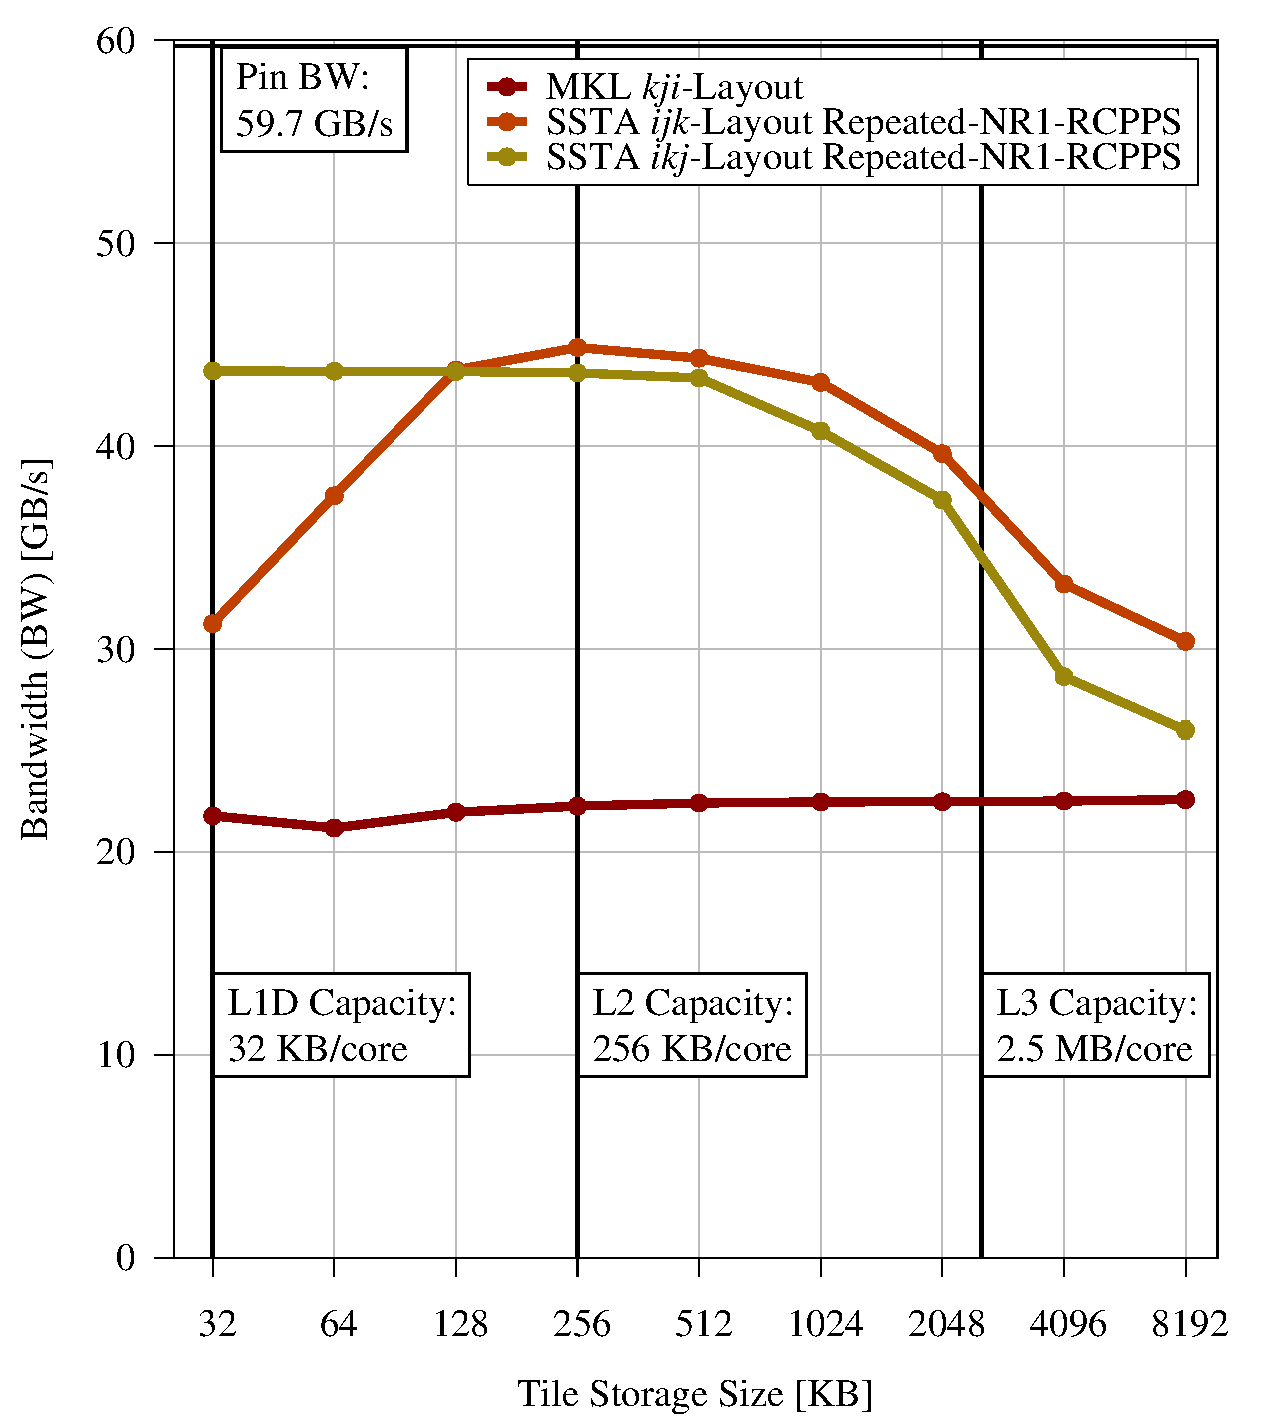
\includegraphics[width=0.99\columnwidth]{figures/post_tsb_tw_sweep_full_matrix_double_precision_production_edison_ivb_e5_2695_v2_08_31_2016_09_03_2016_12pus.pdf}
    \label{fig:results:tile_size_ivb}
  \end{minipage}
  \begin{minipage}{0.49\textwidth}
    \centering
    \caption{
      \textbf{Total Tile Size vs Effective Bandwidth (Haswell):}
      Similar to Figure \ref{fig:results:tile_size_ivb}. 
      \fxnote{Bryce: review?}
    }
    \label{fig:results:tile_size_hsw}
    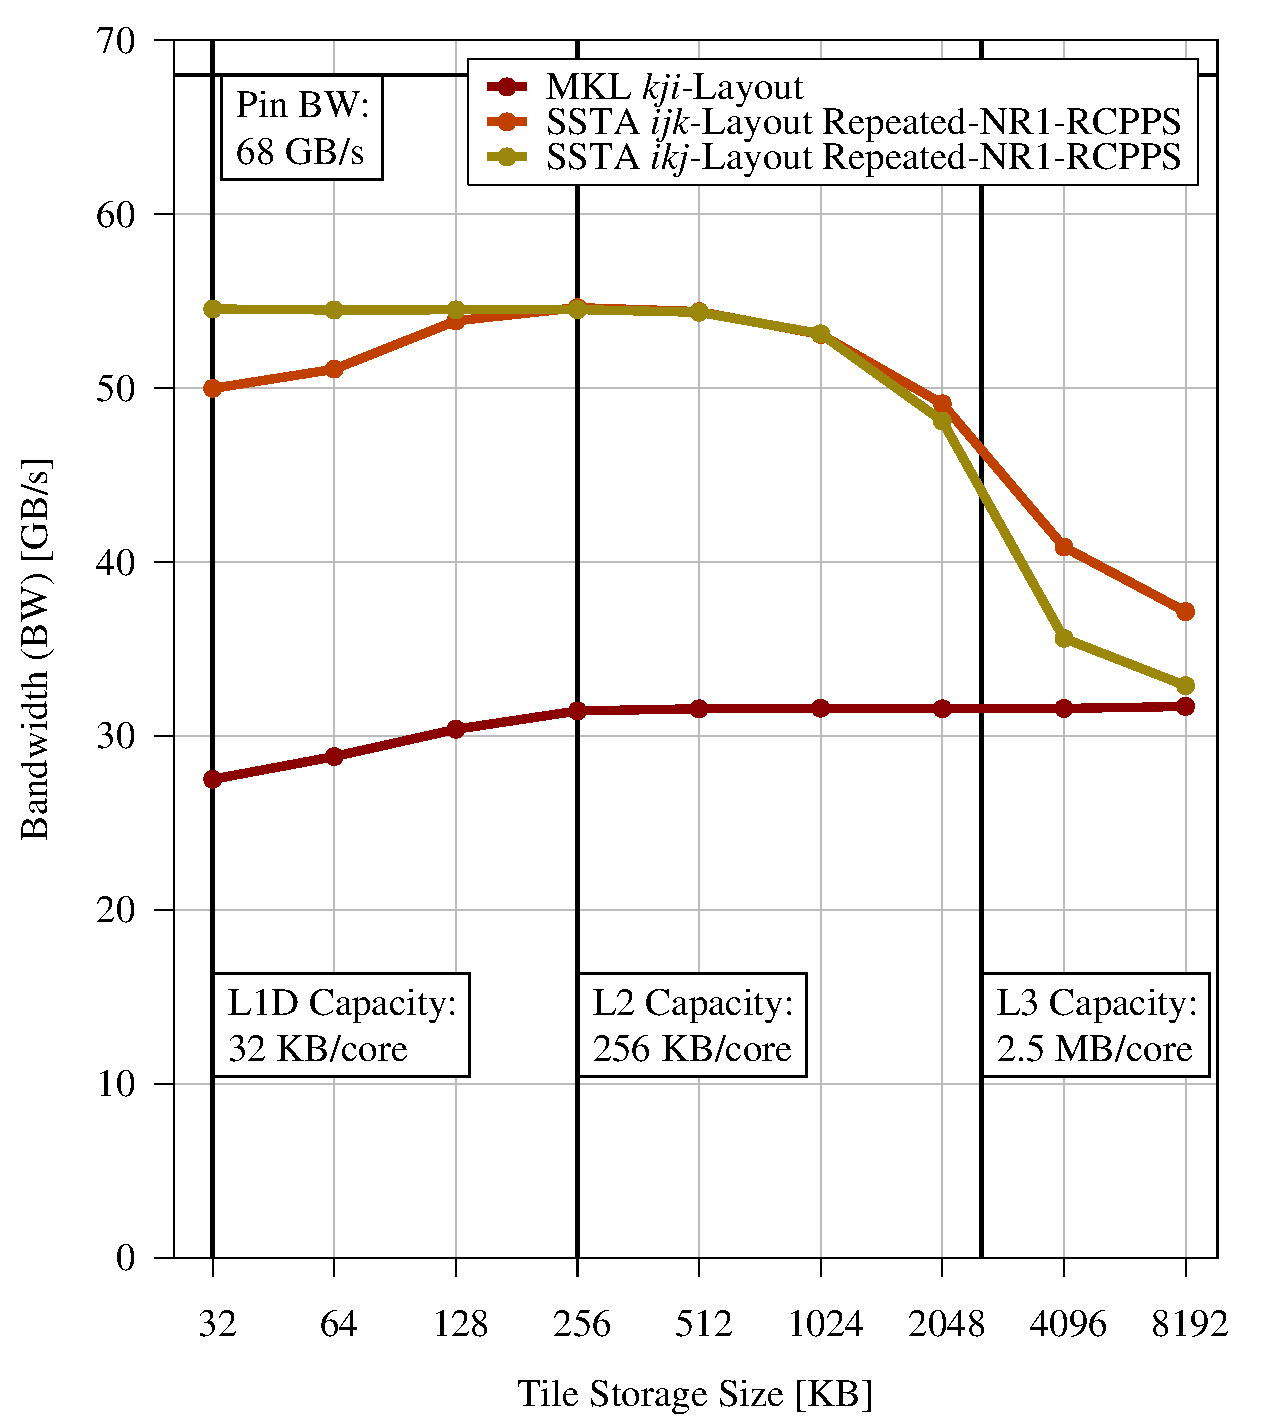
\includegraphics[width=0.99\columnwidth]{figures/post_tsb_tw_sweep_full_matrix_double_precision_production_cori_hsw_e5_2698_v3_08_31_2016_09_03_2016_16pus.pdf}
  \end{minipage}
\end{figure*}

\begin{figure*}[!bth]
  \captionsetup{width=0.39\textwidth}
  \begin{minipage}{0.49\textwidth}
    \centering
    \caption{
      \textbf{Total Tile Size vs Effective Bandwidth (Knight's Landing):}
      Performance of the two variants of TSB, \(kij\)-layout MKL, plotted
      against stream benchmark. Note that MKL achieves less 
      than ${\sim}10\%$ of stream. The TSB approaches show different results: 
      \(ikj\) shows best performance (${\sim}90\%$ of stream) for smallest
      tile sizes that fit in L1 (strong scaling limit), 
      whereas \(ijk\) performance is more consistent (but lower) 
      and best for tiles that fit into L2. The better performance of 
      \(ikj\) potentially due to KNL's long prefetch streaming performance.
      \fxnote{Bryce: review?}
    }
    \label{fig:results:tile_size_knl}
    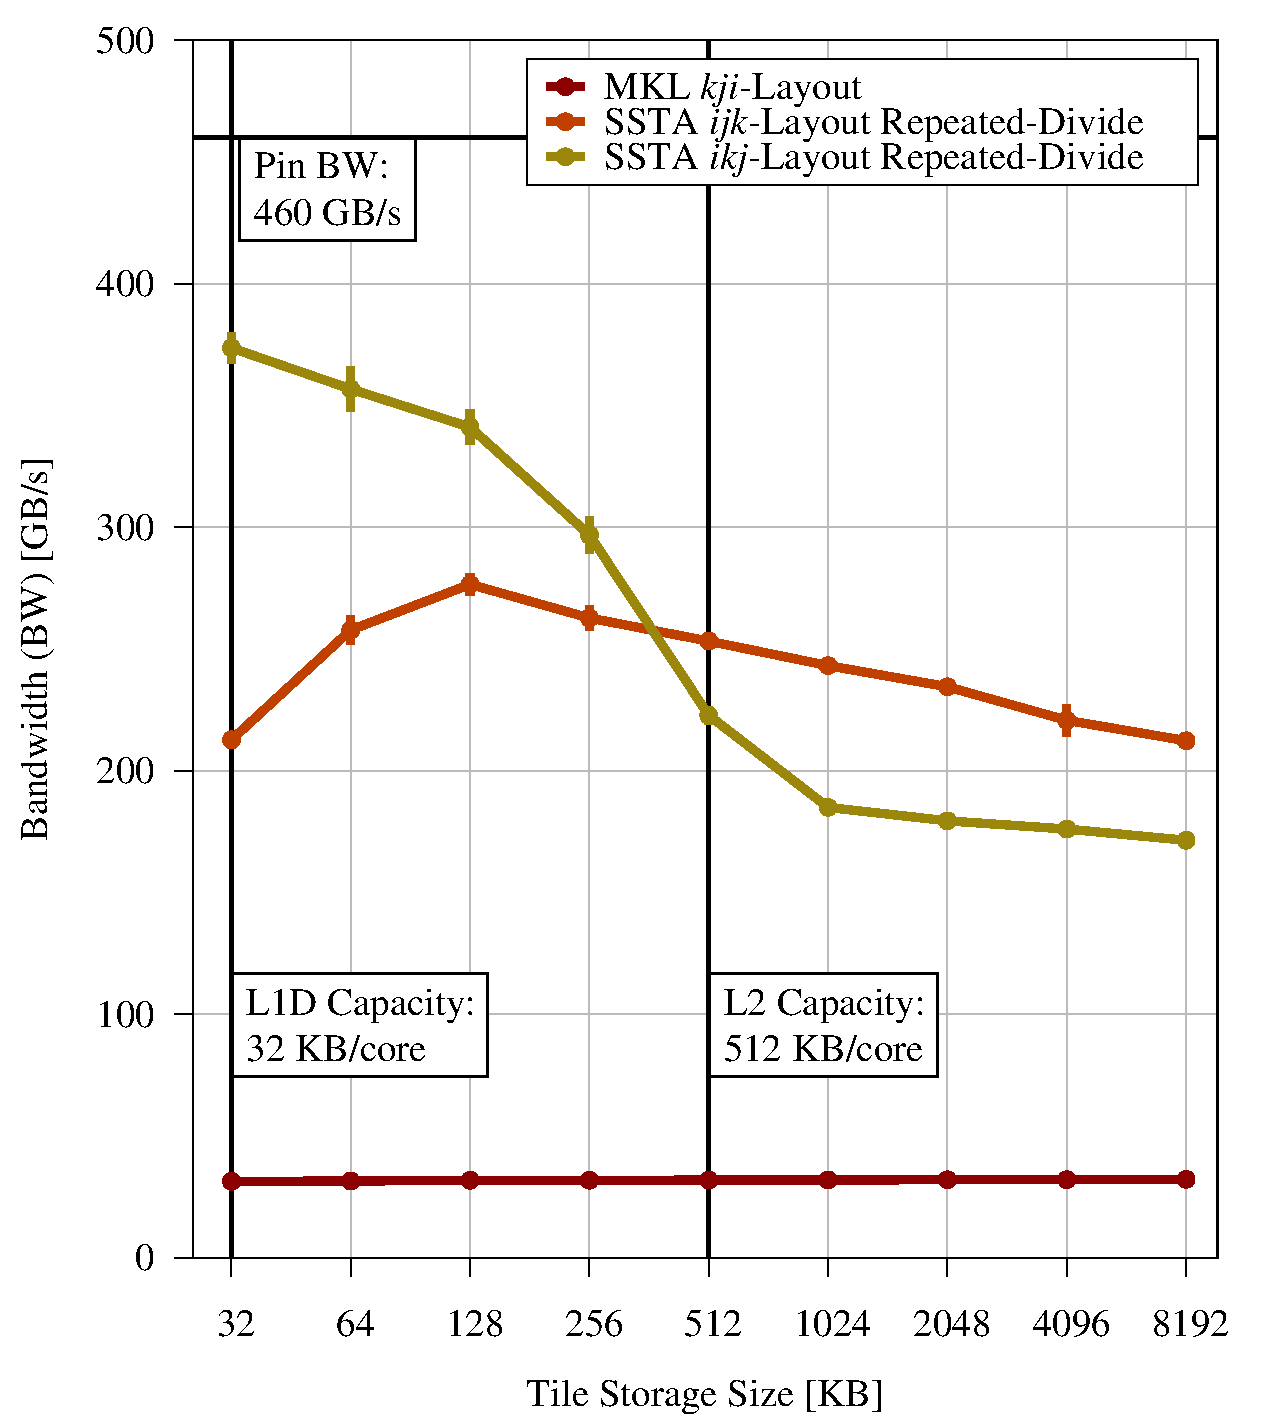
\includegraphics[width=0.95\columnwidth]{figures/post_tsb_tw_sweep_full_matrix_double_precision_production_carl_knl_7210_09_02_2016_64pus.pdf}
    \label{fig:results:tile_size_knl}
  \end{minipage}
  \begin{minipage}{0.49\textwidth}
    \centering
    \caption{
      \textbf{\% of STREAM Triad Effective Bandwidth:}
      Across the three architectures, the TSB algorithm with an optimal 
      tiling size improves over an \(kij\) MKL approach, and achieves
      ${\sim}90\%$ of stream. For KNL, the \(ikj\) layout change is responsible
      for \({\sim}25\%\) of the achieved bandwidth.
      \fxnote{Bryce: review?}
    }
    \label{fig:results:efficiency}
    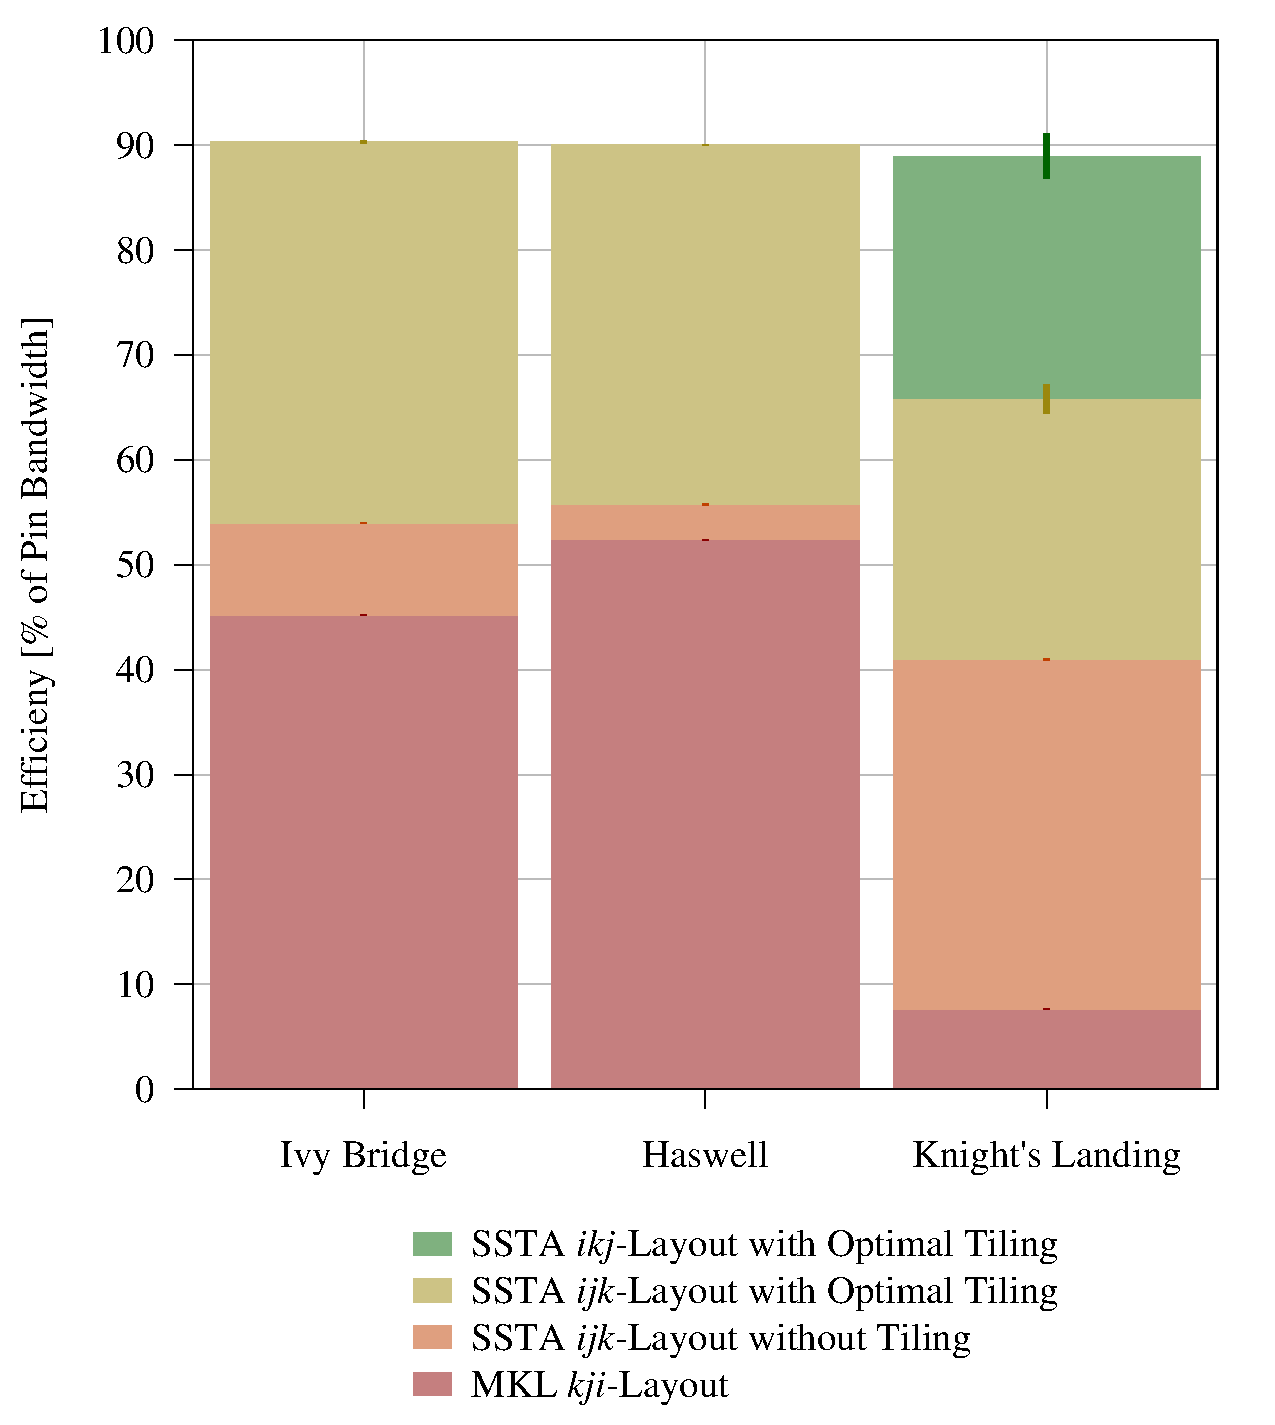
\includegraphics[width=0.95\columnwidth]{figures/post_tsb_impact_of_optimizations_histogram_09_03_2016_09_04_2016_1socket.pdf}
    \label{fig:results:efficiency}
  \end{minipage}
\end{figure*}

% Hypothesis 1.1: SSTA can outperform legacy solver
% Hypothesis 1.2: SSTA can efficiently utilize memory bandwidth 
% Prediction 1.1 and Prediction 1.2 follow naturally 
We developed SSTA to replace the underperforming MKL-based vertical column
  solver in our production climate application because we believed that a new
  algorithm which solves multiple vertical columns simultaneously would
  efficiently utilize available memory bandwidth and significantly outperform the
  legacy solver by exhibiting performant data movement patterns and facilitating
  vectorization.

% Hypothesis 2: SSTA will be highly sensitive to data layout changes and total
% tile size and will achieve optimal performance for a particular tile size
% that balances reuse/locality/amortization.
We also theorized that such a solver would be highly sensitive to
  \textbf{data layout changes} and
  \textbf{total tile size}(\S\ref{sec:implementation:tiling})
Parallel application performance is often driven by parameters such as total
  tile size which control the amount of work in each parallel task.
In memory-bandwidth bound applications, data layout and tiling can be
  especially important as they not only influence the amount of task- and
  vector-parallelism exposed but also the working set size and degree of cached
  data reuse in each individual task.
We anticipated that we would need to study the effect of different data layouts
  and tile sizes in order understand the performance of our new solver.
The first step was to determine the \textbf{optimal total tile size} for the 
  different solver variants in the TSB suite.

%\subsection{Optimal Total Tile Size Parameter Sweep}
%\label{sec:results:tile_size_sweep}

\begin{table*}[t]
  \centering
  \caption{
    \textbf{Performance Comparison of SSTA and MKL Solvers:} \fxnote{Lorem ipsum}
  }
  %%%%%%%%%%%%%%%%%%%%%%%%%%%%%%%%%%%%%%%%%%%%%%%%%%%%%%%%%%%%%%%%%%%%%%%%%%%%%
  \begin{tabular}{|l|r|r|r|r|}\hline
    %%%%%%%%%%%%%%%%%%%%%%%%%%%%%%%%%%%%%%%%%%%%%%%%%%%%%%%%%%%%%%%%%%%%%%%%%%%
      \multicolumn{1}{|c|}{\multirow{2}{*}{\textbf{Solver}}}
    & \multicolumn{1}{ c|}{\textbf{Optimal Total}}
    & \multicolumn{1}{ c|}{\textbf{Effective Bandwidth}}
    & \multicolumn{1}{ c|}{\textbf{Percentage of STREAM}}
    & \multicolumn{1}{ c|}{\multirow{2}{*}{\textbf{Speedup vs MKL}}} \\
    %%%%%%%%%%%%%%%%%%%%%%%%%%%%%%%%%%%%%%%%%%%%%%%%%%%%%%%%%%%%%%%%%%%%%%%%%%%

    & \multicolumn{1}{ c|}{\textbf{Tile Size}}
    & \multicolumn{1}{ c|}{\textbf{Bandwidth}}
    & \multicolumn{1}{ c|}{\textbf{TRIAD Bandwidth}}
    & \\ \hline
    %%%%%%%%%%%%%%%%%%%%%%%%%%%%%%%%%%%%%%%%%%%%%%%%%%%%%%%%%%%%%%%%%%%%%%%%%%%

    \multicolumn{5}{c}{\rule{0pt}{2.25ex} \textbf{Ivy Bridge}} \\ \hline \thickhline
    % BW, Ivy Bridge MKL kji tw_sweep tw=64 results + sig figs
    % % STREAM, Ivy Bridge MKL kji histogram tw=64 results + sig figs
    MKL \(kji\)-layout  &   Any &\(22.49 \pm 0.003\)&\(45.2 \pm 0.05\)& \(1x\) \\ \hline
    % BW, Ivy Bridge SSTA ijk tw_sweep tw=8 results + sig figs 
    % % STREAM, Ivy Bridge SSTA ijk histogram tw=8 results + sig figs
    SSTA \(ijk\)-layout & 256 KB &\(44.0 \pm 0.07\)&\(90 \pm 0.1\)& \(\sim 2x\) \\ \hline
    % BW, Ivy Bridge SSTA ikj tw_sweep tw=1 results + sig figs 
    % % STREAM, Ivy Bridge SSTA ijk PAPER tw=1 results + sig figs
    SSTA \(ikj\)-layout &  32 KB &\(43.0 \pm 0.07\)&\(87 \pm 0.2\)& \(\sim 1.9x\) \\ \hline
    
    \multicolumn{5}{c}{\rule{0pt}{2.25ex} \textbf{Haswell}} \\ \hline \thickhline
    % BW, Haswell MKL kji tw_sweep tw=64 results + sig figs
    % % STREAM, Haswell MKL kji histogram tw=64 results + sig figs
    MKL \(kji\)-layout  &   Any &\(31.65 \pm 0.006\)&\(52.4 \pm 0.04\)& \(1x\) \\ \hline
    % BW, Haswell SSTA ijk tw_sweep tw=8 results + sig figs 
    % % STREAM, Haswell SSTA ijk histogram tw=8 results + sig figs
    SSTA \(ijk\)-layout & 256KB &\(54.3 \pm 0.01\)&\(90.0 \pm 0.07\)& \(\sim 1.7x\) \\ \hline
    % BW, Haswell SSTA ikj tw_sweep tw=1 results + sig figs 
    % % STREAM, Haswell SSTA ijk PAPER tw=8 results + sig figs
    SSTA \(ikj\)-layout &  32KB &\(54.2 \pm 0.01\)&\(89.7 \pm 0.06\)& \(\sim 1.7x\)\\ \hline

    \multicolumn{5}{c}{\rule{0pt}{2.25ex} \textbf{Knight's Landing}} \\ \hline \thickhline
    % BW, Knight's Landing MKL kji tw_sweep tw=64 results + sig figs
    % % STREAM, Knight's Landing MKL kji histogram tw=64 results + sig figs
    MKL \(kji\)-layout  &   Any &\(32 \pm 0.2\)&\(7.6 \pm 0.04\)& \(1x\) \\ \hline
    % BW, Knight's Landing SSTA ijk tw_sweep tw=4 results + sig figs
    % % STREAM, Knight's Landing SSTA ijk histogram tw=4 results + sig figs
    SSTA \(ijk\)-layout & 128KB &\(280 \pm 5\)&\(66 \pm 1\)& \\ \hline
    % BW, Knight's Landing SSTA ikj tw_sweep tw=1 results + sig figs
    % % STREAM, Knight's Landing SSTA ikj histogram tw=1 results + sig figs
    SSTA \(ikj\)-layout &  32KB &\(370 \pm 6\)&\(90 \pm 2\)& \(\sim 12x\) \\ \hline
  \end{tabular}
  %%%%%%%%%%%%%%%%%%%%%%%%%%%%%%%%%%%%%%%%%%%%%%%%%%%%%%%%%%%%%%%%%%%%%%%%%%%%%
  \label{tab:results:comparison}
\end{table*}

%\begin{table*}[t]
%  \centering
%  \caption{
%    \textbf{Optimal Total Tile Sizes:}
%  }
%  %%%%%%%%%%%%%%%%%%%%%%%%%%%%%%%%%%%%%%%%%%%%%%%%%%%%%%%%%%%%%%%%%%%%%%%%%%%%%
%  \begin{tabular}{|l|c|c|}\hline
%    \diagbox[width=10em]{\textbf{Solver}}{\textbf{Platform}} & \textbf{Ivy Bridge \& Haswell} & \textbf{Knight's Landing} \\ \hline
%    MKL \(kji\)-layout  & 2048KB        & 2048KB \\ \hline
%    SSTA \(ijk\)-layout & 128KB - 512KB & 128KB  \\ \hline
%    SSTA \(ikj\)-layout & 32KB - 256KB  & 32KB   \\ \hline
%  \end{tabular}
%  %%%%%%%%%%%%%%%%%%%%%%%%%%%%%%%%%%%%%%%%%%%%%%%%%%%%%%%%%%%%%%%%%%%%%%%%%%%%%
%  \label{tab:results:optimal_total_tile_sizes}
%\end{table*}

We conducted a parameter sweep of total tile size on our Xeon and Xeon Phi 
  platforms.
We predicted that we would see the following: 
\begin{itemize}
% Prediction 2.1: The MKL solver doesn't care about tile size, excluding
% SLOW effects.
\item The MKL baseline solver would be very insensitive to total tile size,
  excluding extremely small (high overhead) and extremely large (insufficient
  parallelism) sizes since it solves each column independently and thus cannot
  exploit locality like the SSTA solver does.
% Prediction 2.2: Total tile sizes which fit in the L1D will be too small to be
% feasible.
\item Total tile sizes small enough to fit into the L1D cache would not be feasible
  because the overheads of loop constructs and parallelization/vectorization
  setup would be too great relative to the execution time of useful work per
  inner-iteration.
These tile sizes would either require vertical extents below the sizes used
  by the applications we are interested in (\(nk < 16\)) or horizontal
  dimensions too small to vectorize efficiently (\(ni < 16\)).
% Prediction 2.3: Optimal total tile size will be in between L1D capacity and
% L2 capacity.
\item The optimal total tile size would fit into the L2 cache (but not the L1D
  cache), since it is the fastest cache which has the capacity to contain a
  tile with a feasible total tile size.
% Prediction 2.4: Performance drops as total tile size crosses cache capacity
% boundaries, excluding L1D.
\item Excluding the L1D, as we move from a tile size which fits into the
  capacity of a particular cache to a tile size which does not, we should see a
  drop in effective bandwidth.
On the Xeon platforms, these boundaries are L2 \(\rightarrow\) L3 and L3
  \(\rightarrow\) DRAM (main memory)
On Knight's Landing, L2 \(\rightarrow\) MCDRAM and MCDRAM \(\rightarrow\) DRAM
  (main memory).
\end{itemize}
Note that when total tile size is equal to a particular cache capacity, we say
  that total tile size will \emph{not} entirely fit into that cache, since it is
  not reasonable to assume that our arrays will be able to consume the entire
  cache's capacity.

The results of this parameter sweep for both the \(ijk\)-layout SSTA variant and
  the \(ikj\)-layout SSTA variant are shown in Figure
  \ref{fig:results:tile_size_ivb} (Ivy Bridge), Figure
  \ref{fig:results:tile_size_hsw} (Haswell) and Figure
  \ref{fig:results:tile_size_knl}.
Results from the TSB suite's MKL baseline solver are shown as a lower bound,
  and STREAM Triad results are shown as an upper bound. 
A \(32 \times 147456 \times 32\) grid of double precision floating point values
  (4.5GB) was used on all platforms.
All results were run on a full socket, with one application-thread per core.

% Analysis of Prediction 2.2: The MKL solver doesn't care about tile size,
% excluding SLOW effects.
We found that the MKL baseline solver was largely insensitive to tile size, as
  anticipated.
Across the range of total tile sizes we tested, we did not observe performance
  variation that was statistically significant enough to distinguish it from
  random experimental error.

% Analysis of Prediction 2.2: Total tile sizes which fit in the L1D will be too
% small to be feasible.
As we predicted, total tile sizes small enough to fit into the L1D cache were
  impractically small.
% Math for exploring tile extents that might fit into L1D
% nj=(32KB*1/2*1/4*1/sizeof(double))*(1/nk)*(1/ni)
%          ^^^ ^^^
%           1   2
% 1: reasonable target working set size 
% 2: # of arrays
We would have to either reduce either the vertical extent or the horizontal
  extent \(ni\) to generate a tile size small enough to fit into the 32KB L1D
  with the tile-\(j\) scheme.
We ran preliminary experiments with \(ni=16\) (not shown) to observe the effect
  of 16KB total tile sizes.
The results indicated that tile sizes smaller than 32KB performed worse for both
  the \(ijk\)- and \(ikj\)-layouts.
At \(ni=16\), the trip count on some of the loops in SSTA is so small that the
  compiler cannot perform as much unrolling after vectorization as it would for
  larger \(ni\)'s.
We have not determined if switching to the tile-\(ij\) scheme might make
  smaller tile sizes feasible without decreasing the extent of the horizontal
  dimension \(ni\) or decreasing performance via worse data contiguity.

% Analysis of Prediction 2.3: Optimal total tile size will be in between L1D
% capacity and L2 capacity.

% ijk Paragraph 1
%For the \(ijk\)-layout, the optimal total tile size is larger than the optimal
%  \(ikj\)-layout total tile size on all platforms.
On Knight's Landing, the optimal total tile size for the SSTA \(ijk\)-layout
  variant is 128K, which is small enough to fit within the L2 but too large
  for the L1D. 
% Knight's Landing tw_sweep tw=4 results + sig figs
%with 95\% confidence that the effective bandwidth is between 265 GB/s and 275 GB/s.
On Ivy Bridge and Haswell, the optimal total tile size for the \(ijk\)-layout 
  is 256KB.
% Roughly 0.16 GB/s gap between the bottom of the 256KB result and the top of
% the next best on Ivy Bridge, roughly equivalent between the 256KB result and
% the next best on Haswell (0.02 GB/s overlap)
While it is difficult to distinguish between the 128KB, 256KB and 512KB results
  in Figures~\ref{fig:results:tile_size_ivb} and~\ref{fig:results:tile_size_hsw}
  because the magnitude of the difference is relatively small, the confidence
  intervals do not overlap and the trend of the dataset supports this conclusion.
% Ivy Bridge tw_sweep tw=8 results + sig figs
% Haswell tw_sweep tw=8 results + sig figs
%We are 95\% confident the best bandwidth for the SSTA \(ijk\)-layout variant is
%  between 43.93 GB/s and 44.07 GB/s on Ivy Bridge and between 54.29 GB/s and
%  54.31 GB/s on Haswell.

% ijk Paragraph 2
We were intrigued to find that, contrary to our predictions, the optimal total
  tile size for the \(ijk\)-layout on the Xeon platforms was too large to fit
  within the L2.
Additionally, while the optimal total tile size for the \(ijk\)-layout on
  Knight's Landing would fit within the L2 cache, performance was not as close to
  peak as it was on the Xeon platforms (\(\sim\) 90\% of STREAM Triad bandwidth
  on both Xeon platforms and between 65\% and 67\% on Knight's Landing; see
  \(ijk\)-layout results in Table \ref{supertable}).
Profiling indicated that the SSTA \(ijk\)-layout variant experienced a high
  number of L1 DTLB store misses.
As we decreased total tile size, we observed progressively worse TLB performance
  in our profiling traces.
We determined this was due to the lack of fully contiguous tiles in the
  \(ijk\)-layout. 
As discussed in \S\ref{sec:implementation:tiling}, tile-\(j\) tiles in the
  \(ijk\)-layout are made up of \(nk\) horizontal \(ij\)-planes. 
As the per-array tile size is decreased, the size of the each contiguous
  regions decreases and the frequency of non-contiguous jumps through memory
  increases, negatively impacting TLB, L1D and hardware prefetching performance
  (especially on Knight's Landing).

% ijk Paragraph 3
We conducted a parameter sweep with the SSTA \(ijk\)-variant and a smaller
  vertical extent (\(nk = 16\), not shown and impractical for production
  applications) to further verify the cause of this issue.
With fewer vertical levels, the number of contiguous regions in each tile would
  be decreased and the size of each contiguous region would be increased, improving
  contiguity.
We observed performance improvements for smaller total tile sizes on the Xeon
  platforms.
On Knight's Landing the impact was much more significant.

% ijk Paragraph 4 (motivation to develop ikj) 
The poor performance of the \(ijk\)-layout at smaller total tile sizes and on
  Knight's Landing led us to develop the \(ikj\)-layout variant of the SSTA
  algorithm described in \S\ref{sec:implementation:data_layout}.
The optimal total tile size for the \(ikj\)-layout was 32KB on all three
  platforms.
On the Xeon platforms, the best \(ikj\)-layout result does not
  outperform the best \(ijk\)-layout result.
However, on Knight's Landing where the best \(ikj\)-layout result achieves
  between 91 GB/s and 109 GB/s higher effective bandwidth than the best
  \(ijk\)-layout result (Figure~\ref{fig:results:efficiency}), a significant
  improvement.

% Summary 
Our prediction that the optimal total tile size would be larger than L1D
  capacity but smaller than L2 capacity held for the \(ikj\)-layout, and for 
  the \(ijk\)-layout on Knight's Landing.
For the \(ijk\)-layout on the Xeon platforms, the optimal total tile size was
  too large to fit into the L2.
We believe the difference between optimal total tile sizes on the Xeon
  platforms and Knight's Landing is due to the lack of a traditional L3 cache on
  the latter, making the performance penalty greater.
We can draw the conclusion that, for the platforms surveyed, the optimal total
  tile size was large enough to reside in the last-level associative on-die cache
  (the L3 on the Xeon platforms and the L2 on Knight's Landing).

% Prediction 2.4: Performance drops as total tile size crosses cache capacity
% boundaries, excluding L1D.
The total tile size parameter sweep somewhat supports our prediction that we
  would see drops in performance as we moved from total tile sizes which would
  fit into a particular cache to tile total tile sizes which would not.
We see no such decrease at the L2 capacity boundary on the Xeon platforms, but
  we do see a drop when the total tile size exceeds L3 capacity per core.
On Knight's Landing, we do see a drop as we cross the L2 capacity boundary.
We posit a modified version of our prediction is more accurate than our initial
  prediction; as we move from a tile size which fits into the last-level
  associative on-die cache, there is a drop in the effective bandwidth of the
  SSTA solver.

%\subsection{Performance Comparison}
%\label{sec:results:comparison}

%\begin{table}[h]
%\centering
%\caption{
%  \textbf{SSTA and MKL Baseline Solver Comparison}: Comparison of the
%    performance of the SSTA and MKL baseline solvers from the TSB suite.
%  The SSTA solver is a substantial performance improvement over the MKL
%    baseline.
%  The results below use the \(ijk\)-layout for SSTA on Ivy Bridge and Haswell,
%    and the \(ikj\)-layout on Knight's Landing.
%  We measured STREAM Triad bandwidth between 49.74 GB/s and 49.86 GB/s on
%    our Ivy Bridge system, between 60.36 GB/s and 60.44 GB/s on our Haswell
%    system and between 418.2 GB/s and 419.6 GB/s on our Knight's Landing system.
%  All measurements are 95\% confidence intervals constructed from the mean and
%    sample standard deviation of multiple samples.
%}
%% FIXME: What does [t] here mean?
%\begin{tabular}[t]{|c|c|c|} \hline
%\textbf{Metric}     & \textbf{SSTA}    & \textbf{MKL} \\ \thickhline
%% BW, Ivy Bridge SSTA ijk tw_sweep tw=8 results + sig figs 
%% BW, Ivy Bridge MKL kji histogram tw=64 results + sig figs
%% % STREAM, Ivy Bridge SSTA ijk histogram tw=8 results + sig figs
%% % STREAM, Ivy Bridge MKL kji histogram tw=64 results + sig figs
%\multicolumn{3}{c}{\rule{0pt}{2.25ex} Intel Ivy Bridge}          \\ \hline \thickhline
%Effective BW [GB/s]   & \(44.0 \pm 0.07\) & \(22.49 \pm 0.003\)  \\ \hline 
%\% of STREAM Triad BW & \(90 \pm 0.1\)    & \(45.2 \pm 0.05\)    \\ \hline
%Speedup vs MKL        & \(\sim 2x\)       & \(1x\)               \\ \hline
%\hline
%% BW, Haswell SSTA ijk tw_sweep tw=8 results + sig figs 
%% BW, Haswell MKL kji histogram tw=64 results + sig figs
%% % STREAM, Haswell SSTA ijk histogram tw=8 results + sig figs
%% % STREAM, Haswell MKL kji histogram tw=64 results + sig figs
%\multicolumn{3}{c}{\rule{0pt}{2.25ex} Intel Haswell}             \\ \hline \thickhline
%Effective BW [GB/s]   & \(54.3 \pm 0.01\)  & \(31.65 \pm 0.006\) \\ \hline 
%\% of STREAM Triad BW & \(90.0 \pm 0.07\)  & \(52.4 \pm 0.04\)   \\ \hline
%Speedup vs MKL        & \(\sim 1.7x\)      & \(1x\)              \\ \hline
%\hline
%% BW, Knight's Landing SSTA ikj tw_sweep tw=1 results + sig figs
%% BW, Knight's Landing MKL kji histogram tw=64 results + sig figs
%% % STREAM, Knight's Landing SSTA ikj histogram tw=1 results + sig figs
%% % STREAM, Knight's Landing MKL kji histogram tw=64 results + sig figs
%\multicolumn{3}{c}{\rule{0pt}{2.25ex} Intel Knight's Landing}    \\ \hline \thickhline
%Effective BW [GB/s] & \(370 \pm 6\) & \(32 \pm 0.2\)             \\ \hline 
%\% of STREAM Triad  & \(90 \pm 2\)  & \(7.6 \pm 0.04\)           \\ \hline
%Speedup vs MKL      & \(\sim 12x\)  & \(1x\)                     \\ \hline
%\end{tabular}
%\label{tab:results:comparison}
%\end{table}

%SSTA was developed to replace an underperforming legacy solver in a production
%  climate code.
%The MKL baseline solver in the TSB suite proxies the performance of the
%  production solver. 
%Our results, summarized in Table~\ref{tab:results:comparison}, show that the
%  SSTA solver delivers significantly better performance than the MKL baseline and
%  should substantially improve the performance of the production code, in line
%  with our predictions

%Our results strongly validate our initial hypothesis that we would be able to
%  outperform our MKL baseline solver and greatly improve utilization of available
%  memory bandwidth.

%===========================================================================
\section{Conclusion}
\label{sec:conclusion}

% Analysis of Prediction 1.1 (can outperform legacy solver)
% Analysis of Prediction 1.2 (can efficiently utilize memory bandwidth)

We introduced the Simultaneous Streaming Thomas Algorithm (SSTA) solver, which
  can solve many small tridiagonal matrix systems simultaneously, a
  problem which arises in a number of scientific application domains.
We have demonstrated the impact of different tiling schemes, total tile sizes
  and data layouts, and how they interact with the memory subsystem.
We showed how our simultaneous solver out performs a natural \(kji\)-layout
  solver.
A parameter sweep demonstrated the sensitivity of the SSTA solver to changes in
  tile size and data layout.
We found that the \(ijk\)-layout version of SSTA provides the best performance
  on Xeon platforms with a total tile size that is small enough to fit into the
  L3 cache capacity per processing-unit but is too large to fit in the L2 cache.
On Knight's Landing, the \(ikj\)-layout yields the best performance with a
  total tile size which is small enough to fit into the L2 cache capacity per
  processing-unit

We have shown that SSTA is a highly efficient solver capable of achieving 90\%
  of STREAM Triad bandwidth on Intel Xeon and Xeon Phi systems, including the new
  Knight's Landing microarchitecture.
Our algorithm is a substantial improvement over the MKL-based legacy solver it
  is designed to replace; it is \(\sim 2x\) faster on Xeon platforms and
  \(\sim 12x\) faster on Knight's Landing.

\section{Future Work}
\label{sec:future_work}

There are a number of future research directions we are interested in exploring
  with the SSTA solver.

There are a number of optimizations which we developed for the SSTA
  solver but have not presented here as they have not delivered the performance
  impact we hoped for.
We developed two optimizations which reduced the number of floating point
  divisions and/or reciprocal estimates that are performed by the SSTA solver. 
The first, the \textbf{cached-divide} optimization, reformulates the Thomas 
  algorithm to remove the division operation from the back substitution loop by
  storing the reciprocal of the temporary value which is written to the array
  \(b\) in the forward elimination loop instead of the temporary value itself.
The second optimization is specific to Intel AVX and AVX2 systems like the Xeon
  test platforms used in this paper.
The AVX and AVX2 extensions provide a single-precision reciprocal instruction
  (RCPPS) but no double precision reciprocal~\cite{intel_opt_manual}.
We developed a vector double-precision division implementation,
  \textbf{NR-RCPPS division}, which converts to single precision, performs an
  RCPPS operation, converts back to double precision and then performs Newton
  Raphson iterations.
While we found both optimizations to be beneficial in serial, they decreased
  performance if combined together and had little impact in parallel.
We also experimented with a technique to mitigate cache aliasing
  conflicts, but we were not able to distinguish a clear performance impact.

The version of the TSB suite described in this paper uses what we refer to as
  the \textbf{full-grid} scheme, where the tridiagonal matrix is built and stored
  for all vertical columns and we do not include the construction of the matrix
  in our measurements or performance model.
The alternative, the \textbf{rolling-grid} scheme, builds the matrix on the fly
  with a tile-sized, \lstinline{thread_local} \(a\), \(b\) and \(c\).
In addition to offering storage savings, we believe the rolling-grid scheme
  will further improve data locality and hardware prefetching performance as the
  storage for the matrix will be the same for all tiles which each thread
  executes.
However, this technique requires building the matrix within the
  OpenMP-parallelized tile loop which we time.
Due to the short duration of each individual tile solve, it is not possible to
  time each individually with our current timing mechanism.
It is possible that we might be able to perform such timings with our other
  timing mechanism, which utilized a hardware timestamp counter (e.g.
  RDTSCP~\cite{intel_opt_manual}).
Alternatively, we could incorporate the matrix build into our performance
  model, although this would decrease the overall AI of SSTA.
Further research is needed to explore smaller total tile sizes, as well as the
  tile-\(ij\) scheme further as it may be beneficial to production applications
  that are willing to accept some performance trade-off for increased flexibility
  in the extent of the horizontal extent \(ni\).

We would like to extend the range of hardware platforms and configurations in
  future experiments.
We have not yet fully investigated the utilization of hyper-threads with the
  SSTA solver.
Additionally, we have primarily used MCDRAM as a direct-mapped, hardware
managed cache on Knight's Landing.
Further effort is needed to study the trade-off between utilizing on-package,
  high-bandwidth memory as a cache versus programmable memory which must be
  allocated with a special interface.
We are also interested in testing the SSTA solver on SIMT GPGPU
  architectures.

There are also a number of related numerical problems which we believe could be
  addressed by some of the techniques we describe in this paper.
The existing algorithm is directly applicable to block-tridiagonal matrices,
  where diagonal and off-diagonal blocks can be solved simultaneously
  to accelerate larger, distributed matrix solves.
% Bryce: I'm hesitant to say anything about tiling \(k\) with a Thomas-algorithm
% type solve, I just don't know enough about it. There are loop-carried dependencies
% so I'm not sure you'll get anywhere producitivity 
%This would also be the basis for better strong scaling by tiling in
%  the vertical \(k\) direction as well, and potentially smaller
%  tile sizes overall. 
The current algorithm needs to be extended to include matrix assembly
  based on solution values, and put inside a fully non-linear iteration
  with a Jacobian calculation, such as used in Newton iterations.
The challenge here is that some vertical columns may converge faster than
  others, and vector masks or scalar iterative refinement may be required.
Opportunities to extend the algorithm to banded matrices and incomplete LU-type 
  algorithms are straight-forward for diagonally-dominant cases, but
  pivoting has the potential to hinder vectorization if not carefully
  implemented.

Finally, more complex applications integrate multiple solvers and
  computationally phases, such as traditional ``stencil'' finite difference
  operations and time integration algorithms. 
It remains to be seen if there are
  performance trade-offs between \(ijk\)-layout and \(ikj\) in these
  applications.
% Closer.
Our efforts in the immediate future will revolve around integration of the SSTA
  solver into our production software and research into those trade-offs.

%===========================================================================
%\section*{Acknowledgments}
%
%This material is based upon work supported by the U.S. Department of Energy, Office of Science, Advanced Scientific Computing Research, Scientific Discovery through Advanced Computing (SciDAC) program.
%This work was partially supported by the Intel Parallel Computing Center at
%Lawrence Berkeley National Laboratory,
%and used resources at the National Energy Research Scientific Computing Center, which are supported by the U.S. Department of Energy Office of Science's Advanced Scientific Computing Research program under contract number DE-AC02-05CH11231.  
%This research used resources in Louisiana State University's Center for Computation and Technology. 
%\fxnote{Bryce: Check with Adrian if there's wording here that LSU likes}

%This research used resources of the National Energy Research Scientific Computing Center (NERSC), which is supported by the Office of Science of the U.S. Department of Energy under contract DE-AC02-05CH11231.
%This research used resources of the Argonne Leadership Computing Facility at Argonne National Laboratory, which is supported by the Office of Science of the U.S. Department of Energy under contract DE-AC02-06CH11357.
%This research used resources of the Oak Ridge Leadership Facility at the Oak Ridge National Laboratory, which is supported by the Office of Science of the U.S. Department of Energy under Contract No. DE-AC05-00OR22725.


%===========================================================================
\bibliographystyle{IEEEtran}
\bibliography{sc16-implicit}
%===========================================================================

%===========================================================================
% 

%\section*{Notes/Outline}
%Submission info:
%\url{https://easychair.org/conferences/?conf=pmbs16}
%
%\begin{itemize}
%\item Climate apps use HE-VI model 3D+1D. Also a pattern for 2D+1D and 3D+0D chemistry
%\item Results demonstrate importance of ``batching'' solves, MLK doesn't do
%\item Cache coherency is important: IMEX RK accum, tiling
%\item Explicit part is HO stencil op, memory b/w bound (w/ ghost cells)
%\item Implicit part is non-linear solver: App requires different matrix at each i,j index 
%\item Results in repeated vertical sparse banded solve
%\item Solve (tridiag, banded, dense) should vectorize on i (unit stride), tiled in pencils
%\item Considerations for vector alignment, tiling, and memory
%\item Performance results, scaling, comparison, by platform / parameter
%\item Future work: communication hiding, load imbalance, IMEX
%\end{itemize}
%(Bryce's email comments) Looking over the outline:
%\\
%It's crucial that we clearly identify the optimizations that we
%believe are novel/high-impact, vs the optimizations that are
%well-known to the community (even if they were not well known to us).
%For example, on the outline, we have listed "IMEX RK accum, tiling".
%Do we want to present the accumulation optimizations which removed
%unnecessary temporaries from the time integrator? Do we feel that
%optimization is novel, or is that just a common-sense thing that only
%affected us because of the Chombo programming model? Likewise, do we
%want to present tiling as a focal point in this paper? Tiling is a
%well-known technique; we certainly can't claim tiling in general as
%novel work. Is some part of our tiling approach novel? (how about
%parallelizing the tile loop - is that fairly novel? I know Sam does
%this in HPGMG, but is this a widely used technique?)
%\\
%We would be well served by applying the scientific method at this juncture:
%\\
%\begin{itemize}
%\item Question: What concrete research question(s) are we answering?
%\begin{itemize}
%\item Prior research indicates that HE-VI methods show promise as a
%scalable approach to solving global climate problems on cubed sphere
%geometries because <explanation> [cite prior studies]. How do we
%implement HE-VI methods which perform well on cache-coherent SIMD
%architectures?
%\item When solving a problem with a high horizontal-vertical aspect ratio
%(e.g. the horizontal extents are much greater than the vertical
%extents) with HE-VI methods, it is necessary to perform a large number
%of small vertical implicit solves (<give examples of matrix sizes>
%[citation]) which are independent of each other. <explain the type of
%solves in the climate dycore - e.g. non-linear but nearly banded>
%[citation]. How can we efficiently solve large quantities of small
%non-linear bandedish/banded/tridiagonal matrices on cache-coherent
%SIMD architectures?
%\end{itemize}
%\item Hypothesis: What theories did we come up with that would answer our
%research question(s)?
%\begin{itemize}
%\item Optimal memory access patterns, management of working set sizes
%(e.g. staying in cache) and efficient use of vector units are
%necessary to achieve good performance on cache-coherent SIMD
%architectures.
%\begin{itemize}
%\item Optimal memory access patterns: moving through memory in unit
%stride, controlling the number of streams.
%\item Management of working set sizes: tiling, reducing size of
%temporaries/localizing temporaries (thread-local or otherwise)
%\item Efficient use of vector units: moving through memory in unit
%stride, controlling memory alignment, controlling array strides,
%annotation-assisted autovectorization
%\item TODO: List of individual, concrete optimizations from above.
%\end{itemize}
%\item Mainstream linear algebra libraries (<examples> [citation]) are not
%well-suited for solving large quantities of small non-linear
%bandedish/banded/tridiagonal matrices on cache-coherent SIMD
%architectures because <expalanation> [cite prior studies if possible].
%\end{itemize}
%
%
%\item Prediction: If our hypotheses are true, what results can we expect to
%see? \\
%$\rightarrow$ TODO: What performance characteristics should we see with and
%without each of the concrete optimizations from our hypothesis above?
%
%\item Experiment: Investigate the predictions we've made. \\
%$\rightarrow$ TODO: Methodology for benchmarking the optimizations identified
%above and measuring the performance characteristics we're interested
%in.
%
%\item Analysis: What were the results of our experiments?
%\end{itemize}
%
%List of figures from meeting on 8/11:
%For KNL, HSW, SNB(?)...
%List of figures from meeting on 8/11:
%-For KNL, HSW, SNB(?)...
%\begin{enumerate}
%\item Baseline performance using MKL (and hand) using i-major data layout 
%(not vectorized)
%\item Performance as a function of 32b RCP NR (not needed on KNL), stored
%reciprocal (cuts divides in half) for fixed file size (4?)
%\item Performance vs. Tile Size (jtile = 1,2,4,8,16,32)
%\item Best Performance vs. MKL using same data layout vs. MKL using its best
%(include DRAM BW limit)
%\item Performance as a function of total parallelism for constant tile size
%[optional time permitting]
%\item Performance with 2,3,4 hyperthreads...  maybe just prose comments?
%\item effect of kdim != pow(2)... maybe just prose comments?
%\end{enumerate}
%\newpage
%\section*{TODO}
%
%\fxnote{from SAM: I think the paper/abstract should respond to a few points in 
%their topics of interest...}
%\begin{itemize}
%\item Performance evaluation and lessons learnt \\
%  == Early/First examination of KNL for climate codes
%\item Extensions to and shortcomings of current accelerator directives APIs \\
%  == some comment on observation that compilers are unable to see beyond OMP on
%a column and realize a loop transformations (for vectorization) across multiple
%columns can be performed.
%\item Auto-tuning and optimization strategies \\
%  == tuning tile sizes / caching divides / etc...
%\end{itemize}
%
%\fxnote{HANS: Most of the length is due to two competing goals for the paper: 
%  an optimization process, or a benchmark. Skip the benchmark for now \dots}
%
%\fxnote{SAM/HANS: is anything learned from single-core results here? Drop?}
%
%\fxnote{HANS: where is the discussion of how the B/W is calculated? 
%  Where are the wallclock times?}


%\begin{figure*}
%\listoffixmes
%\end{figure*}

\end{document}


